% \documentclass[../main.tex]{subfiles}

% \begin{document}
% \Blindtext
% \end{document}
\section{Work Done}

\label{work_done}
% \noindent

\subsection{Overview of the Work Done}
The overview of the work done is as follows:
\begin{itemize}
	\item A stable consistent region selection procedure is proposed using GLCM
	      and statistical features to extract features invariant to sensor errors.
	\item Combination of different types of feature vectors gives an edge over
	      the existing methods to obtain an irreversible and stable key from the
	      fingerprint of a user.
	\item The proposed method works well over images of varying quality and
	      resolution. The approach is robust, produces accurate results and is tested
	      thoroughly with several fingerprint biometric datasets
	      (\cite{maio2002fvc2002}, \cite{maio2004fvc2004}, \cite{polyu2016database}).
	\item The keys generated according to the proposed approach passed
	      statistical tests like NIST tests~\cite{pareschi2012statistical} and Diehard
	      tests~\cite{marsaglia1998diehard} successfully, thus ensuring randomness.
	\item The proposed method is a simple technique for dynamic and scalable key
	      generation which does not require complex hardware and is computationally
	      inexpensive.
	      %\item We have proposed a secure and efficient technique to transfer
	      %the confidential dataset credentials from "dataset owner" to
	      %"research student" using our key (as private key).
\end{itemize}

\subsection{Proposed Approach}
This section enlists the proposed approach of key generation using a
fingerprint image. An overview of the proposed approach is shown in
Fig. \ref{fig:blockdiagram}. The approach is divided into several modules. The
objectives and details of each module are as follows:

\begin{itemize}
	\item \emph{Pre-processing:} A biometric data captured in an uncontrolled
	      the environment is usually riddled with noise and has an improper alignment.
	      Standard pre-processing procedures for image enhancement and alignment is carried out to deal with such input.
	\item \emph{Consistent region selection:}  In addition to noise, another
	      problem with the input is the partial capturing of the fingerprint. A
	      part of the input image is chosen meticulously to deal with this
	      problem so that the region is consistent in most of the input data.
	\item \emph{Hybrid feature extraction:} In this step, a feature set is
	      extracted from the consistent region.
	\item \emph{Prominent feature selection:} Extracted features are optimized
	      to generate a stable feature vector.
	\item \emph{Discriminant feature vector generation:} In order to make the
	      key-generation process robust and reliable,
	      the discriminant feature vector is extracted from the prominent features.
	\item \emph{Key generation:} Finally, the key is generated from the
	      discriminant feature vector.
\end{itemize}

\begin{figure}[!ht]
	\centering
	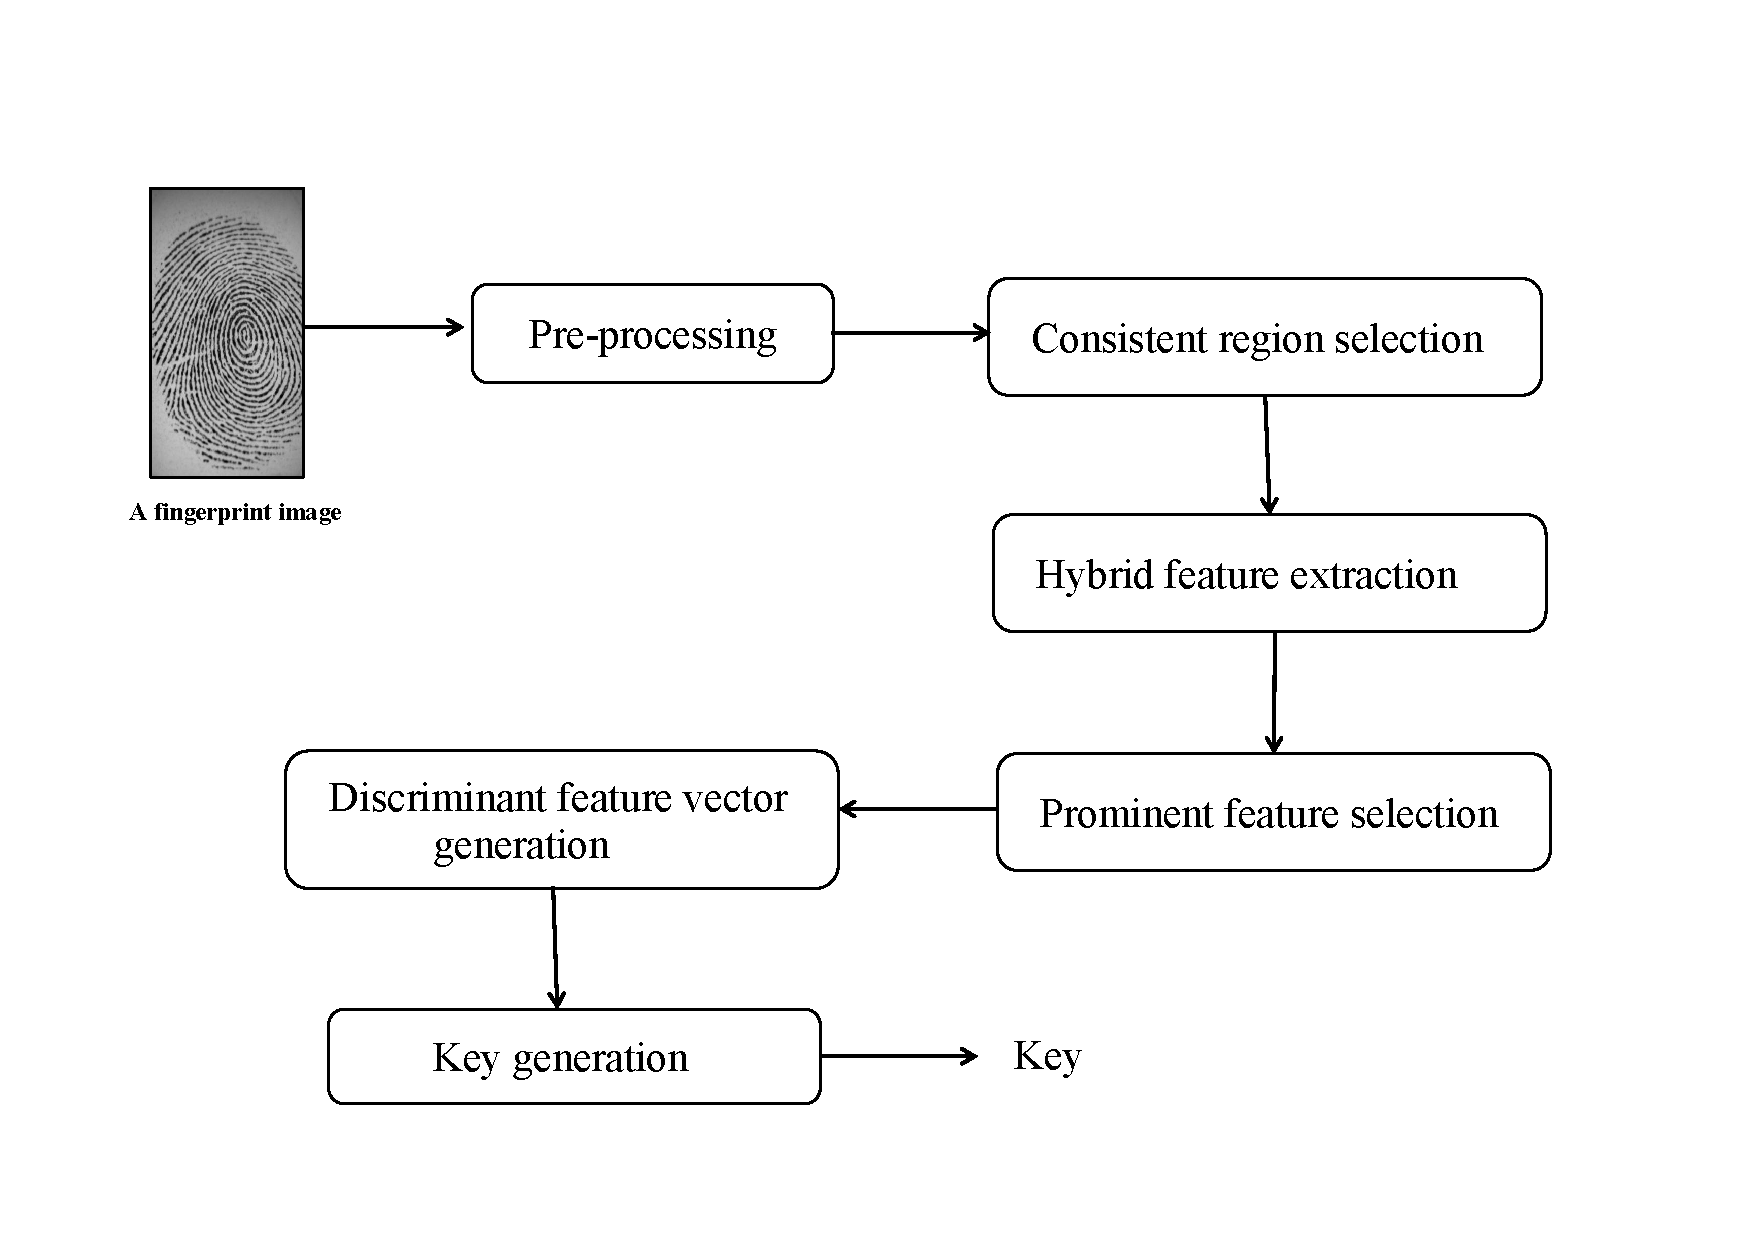
\includegraphics[width=2.5in]{blockdiagram.pdf}
	\caption{Overview of the key generation from a fingerprint image.}
	\label{fig:blockdiagram}
	% \vspace{-6mm}
\end{figure}



\subsubsection{Pre-processing}
The pre-processing step is crucial for stable feature extraction from a
fingerprint image. Level-2 features such as the minutiae feature extraction
depend heavily on accurate and standard pre-processing steps. The
pre-processing steps consist of robust and accurate segmentation, alignment,
and enhancement procedures.

\par

This work adopts factorized directional bandpass
(FDB) segmentation~\cite{thai2016filter} technique to extract the fingerprint
region from a fingerprint image. This segmentation technique helps in vertically
aligning the rotated fingerprint effectively. Next, ASRA alignment
technique~\cite{Faguletal} has been implemented to align the input fingerprint
vertically. Finally, the fingerprint image is enhanced using the method
proposed by Ding et al. \cite{ding2017combining}. A sample pre-processed
fingerprint is shown in Fig.~\ref{fig:pre-processing} as an illustration.

\begin{figure}[!ht]
	\centering
	\subfigure[Original fingerprint image.]{
		\centering
		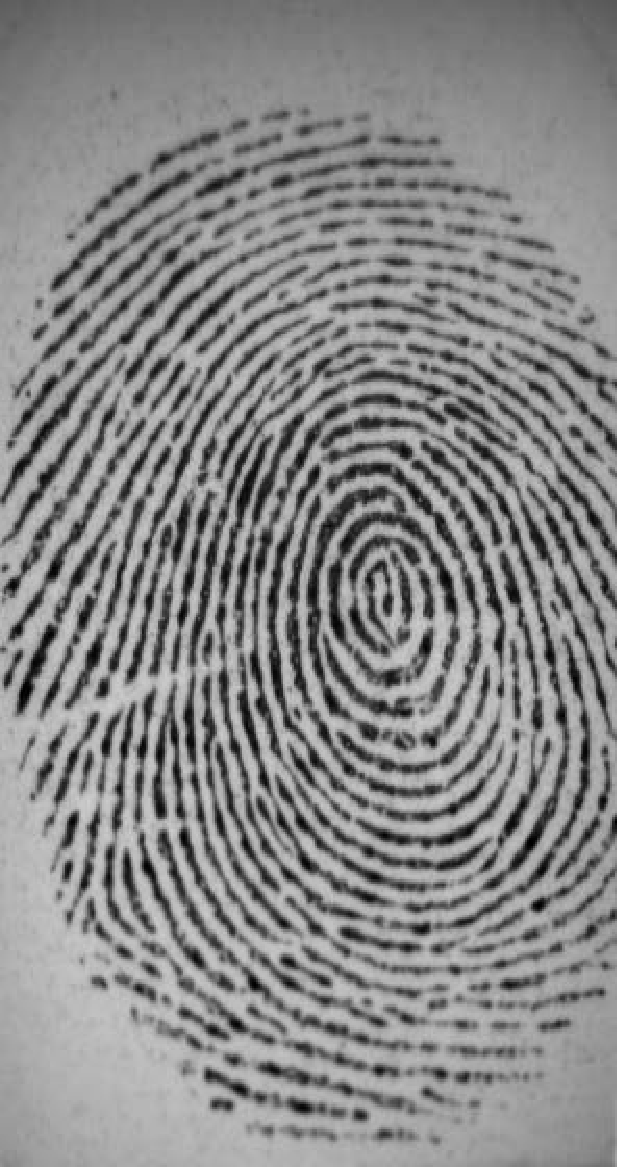
\includegraphics[width=0.5in]{images/pre-proc_1.pdf}
		\label{fig:original}} \subfigure[Vertically aligned image.]{\centering
		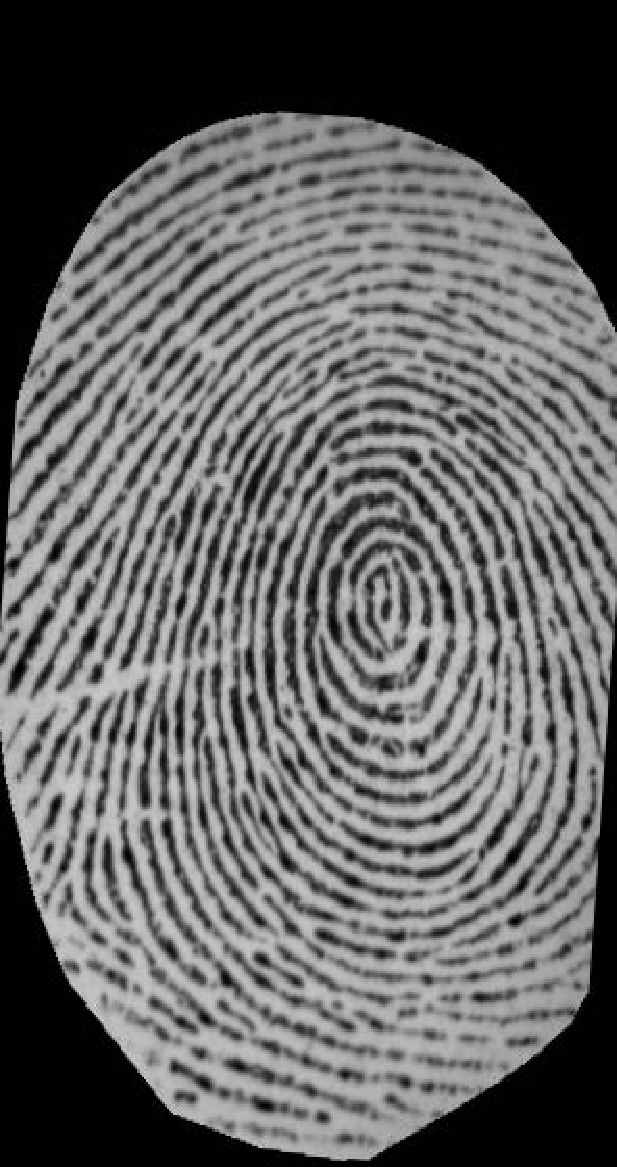
\includegraphics[width=0.5in]{images/pre-proc_2_rotated.pdf}
		\label{fig:aligned}} \subfigure[Enhanced image.]{\centering
		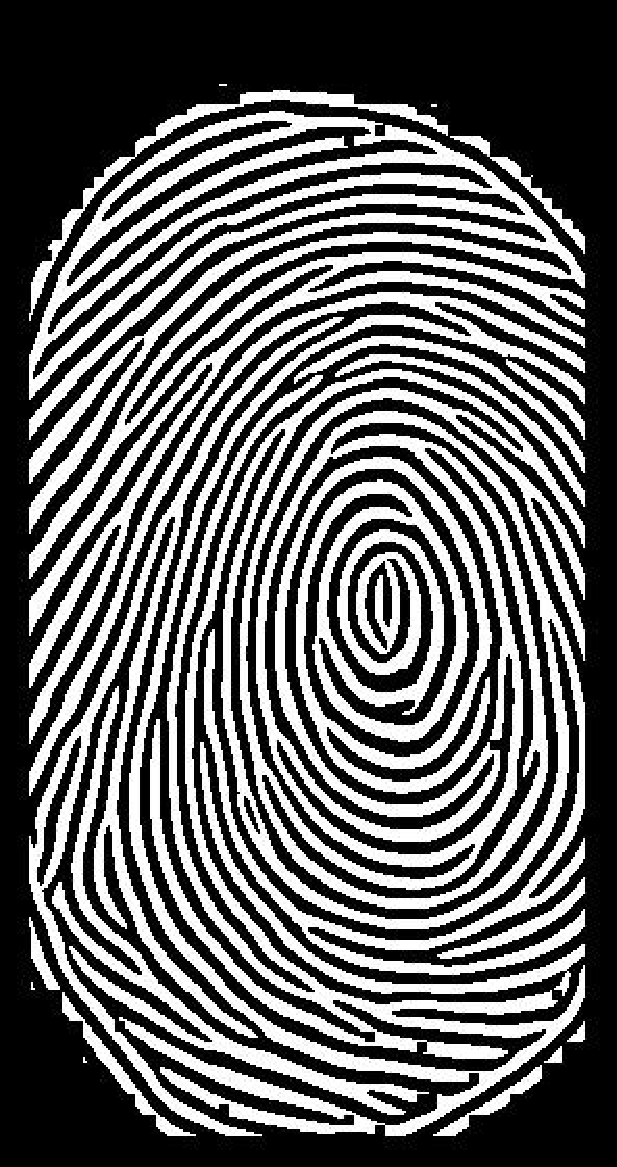
\includegraphics[width=0.5in]{images/pre-proc_3_enhanced.pdf}
		\label{fig:Enhanced}}
	\caption{An illustration of pre-processing of a sample fingerprint image.}
	\label{fig:pre-processing}
	\vspace{-4mm}
\end{figure}

\subsubsection{Consistent region selection}
The entire fingerprint not necessarily contribute evenly for robust feature
extraction. The consistent region is selected from the fingerprint to obtain
efficient features that can increase recognition accuracy. In this work, both
Gray Level Co-occurrence Matrix (GLCM) \cite{garg2020novel} and statistical
features-based approaches are followed to determine the consistent region of an
image. The procedure consists of the following concepts.
\subsubsubsection{ Gray Level Co-occurrence Matrix (GLCM) and statistical features}
GLCM is a popular technique known for the extraction of texture-based features in an
image ~\cite{garg2020novel}. This method estimates the relative position of
pixels in a neighborhood by calculating the statistical properties of the image.
\begin{figure}[!ht]
\centering
	\subfigure[GLCM calculation example for value pairs (0,1), (1,1) and (3,2)
		in the offset direction $0^o$.]{
		\centering
		% include first image
		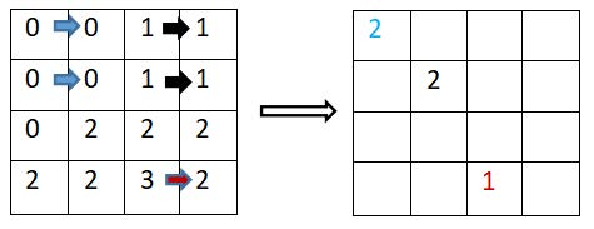
\includegraphics[width=2.0in]{images/glcm_2.pdf} }
	%\caption{Put your sub-caption here} \label{fig:sub-first} \end{subfigure}
	\subfigure[GLCM co-occurrence matrix.]{
		\centering
		% include second image
		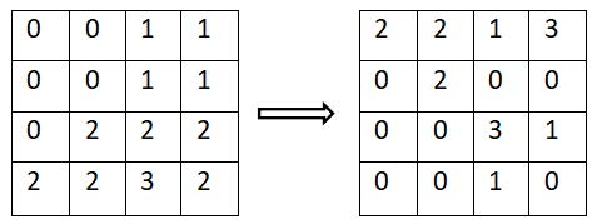
\includegraphics[width=2.0in]{images/glcm_3_final.pdf}}
	\hfil
	\subfigure[GLCM matrix calculation along four directions with offset two.]{
		\centering
		% include second image
		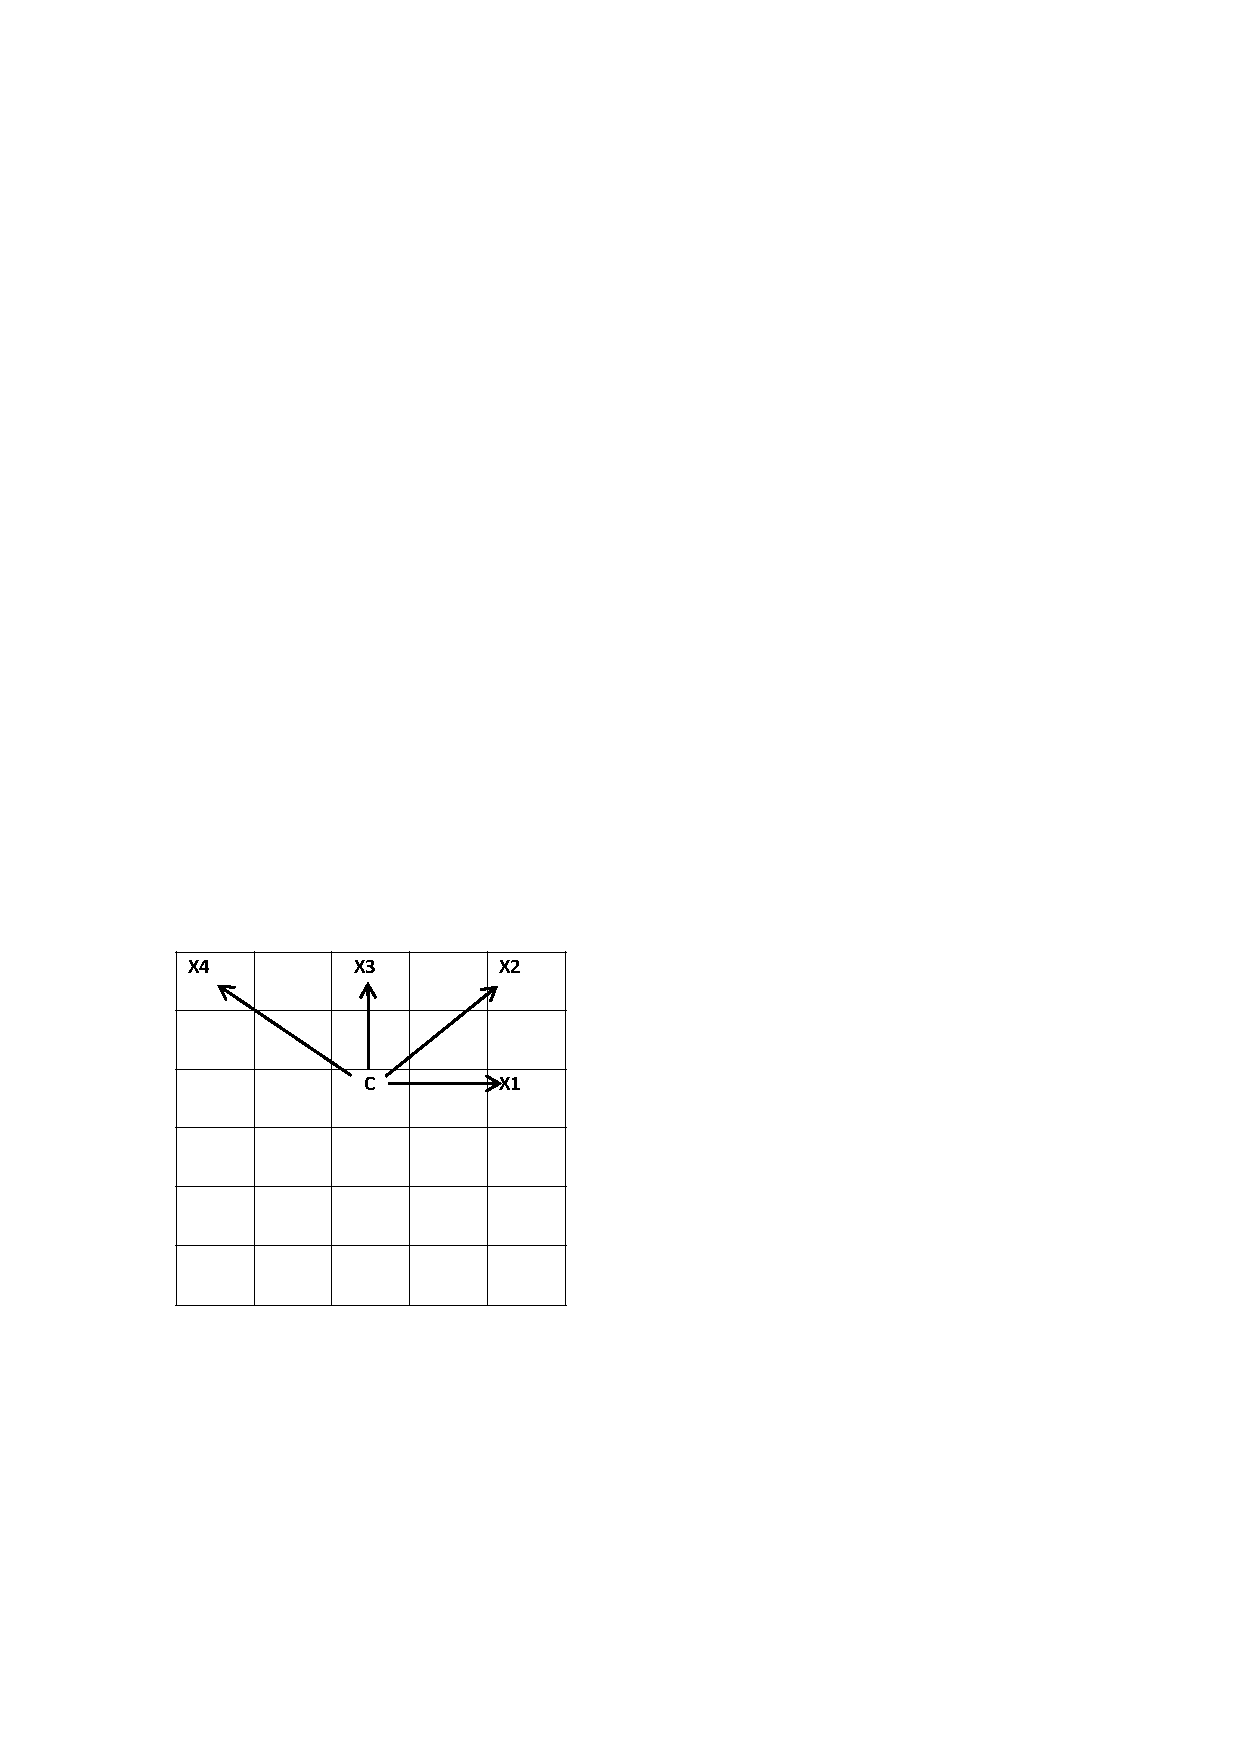
\includegraphics[width=0.7in]{images/glcm_1.pdf}}
	\caption{An illustration of GLCM feature extraction.}
	\label{fig:GLCM}
\end{figure}

In this method, a co-occurrence of a matrix $C$ is calculated as
\begin{equation}\label{glcm}
	\begin{split}
		C_{\Delta m,\Delta n}(x,y)=\sum_{i=1}^{M-\Delta m}\sum_{j=1}^{N-\Delta n}\left\{\begin{matrix}
			1 & if~I(i,j)= x, I(i+\Delta m, j+\Delta n)= y \\
			0 & Otherwise
		\end{matrix}\right.
	\end{split}
\end{equation}
where $I(i,j)$ is the intensity of an image at position $(i,j)$. Image size is
$M \times N $. The vector v=$(\Delta m, \Delta n)$ covers 4 directions $(D1, D2,
	D3, D4)$ in an image. The working of GLCM process is shown in Fig.
~\ref{fig:GLCM}.

From the GLCM matrix, three statistical features, namely Correlation,
Homogeneity and Energy are obtained using Equations
\ref{glcm_Correlation},~\ref{glcm_homogenity} and \ref{glcm_energy},
~respectively.

\noindent \textbf{Correlation:}\\Returns a measure of how correlated a pixel is
to its neighbor compared to the whole image.
\begin{equation}\label{glcm_Correlation}
	C\_Correlation= \sum_{x} \sum_{y} \frac{(x-\mu_{x})\cdot(y-\mu_{y})\cdot C(x,y)}{\sigma_{x}\cdot \sigma_{y}}
\end{equation}
\noindent \textbf{Homogeneity:}\\Returns a value that measures the closeness of
the distribution of elements in the GLCM(C) to the GLCM(C) diagonal.\\
\begin{equation}\label{glcm_homogenity}
	C\_Homogeneity= \sum_{x} \sum_{y} \frac{C(x,y)}{1+|x-y|}
\end{equation}\\
\vspace{2pt}
\noindent\textbf{Energy:}\\Returns the sum of squared elements in the GLCM(C).
\begin{equation}\label{glcm_energy}
	C\_Energy= \sum_{x} \sum_{y} C(x,y)^{2}
\end{equation}
\subsubsubsection{Consistent region selection based on GLCM statistical feature descriptor}
The proposed consistent region selection method uses GLCM statistical feature
descriptor followed by a classification and k-fold validation step. The steps
are as follows:
\begin{itemize}
	\item \textbf{Step-1}: An input fingerprint image $I$ is duplicated into
	      four instances.
	\item \textbf{Step-2}: For each fingerprint instance, a central point  $o$
	      is determined. Let the core point in $I$ be the central point $o$.
	      Next, $64\times 64 $  region around the central point $o$ is selected.
	      Let the region be denoted as $r$.
	\item \textbf{Step-3}: For the region $r$ in each fingerprint instance, the
	      GLCM matrix $C$ is calculated using Equation \ref{glcm}. The feature
	      descriptor is derived using Equations \ref{glcm_Correlation},
	      \ref{glcm_homogenity} and \ref{glcm_energy}, respectively. Let the
	      feature vector be called $f$, where $f=[f_{Correlation},f_{homogenity},f_{energy}]$ of
	      length $12$.~The features are calculated along four directions
	      $(0^{0}, 45^{0}, 90^{0}, 135^{0})$ and with different pixel offsets
	      ($1,2,\ldots,10$). ~If there are 10 individuals in the dataset, each
	      having 8 instances, then 4 instances of each user is used in this
	      step. The feature vectors derived for all four instances for all
	      individuals is combined into one vector (denoted as $F$). The
	      resultant vector $F$ has dimension $40 \times 120$.
	\item \textbf{Step-4}:~One-vs-all SVM is applied on $F$ with k-fold
	      cross validation (k=10).~The prediction accuracy, $A_{t}$, is calculated
	      by averaging the accuracy obtained from all $k$ folds.
	\item \textbf{Step-5}:The region $r$ (from Step 1) of each instance in the fingerprint
	      is scaled up 1.2 times (decided empirically). Steps $2$, $3$ and $4$
	      are repeated until $A_{t+1} \leq A_{t} $ (where, $t$ is the
	      iteration number) %The prediction accuracy($A_{t+1}$) is calculated.
	\item \textbf{Step-6}:The resultant $r$ is the required consistent region.
\end{itemize}

For a query image, this region $r$ is used as a reference around central
point to select the consistent region.~The consistent region selection is shown
in Fig. \ref{fig:consistent}.
\begin{figure}[!ht]
	\centering
	\subfigure[Original ROI $r$ around central point.]{
		\centering
		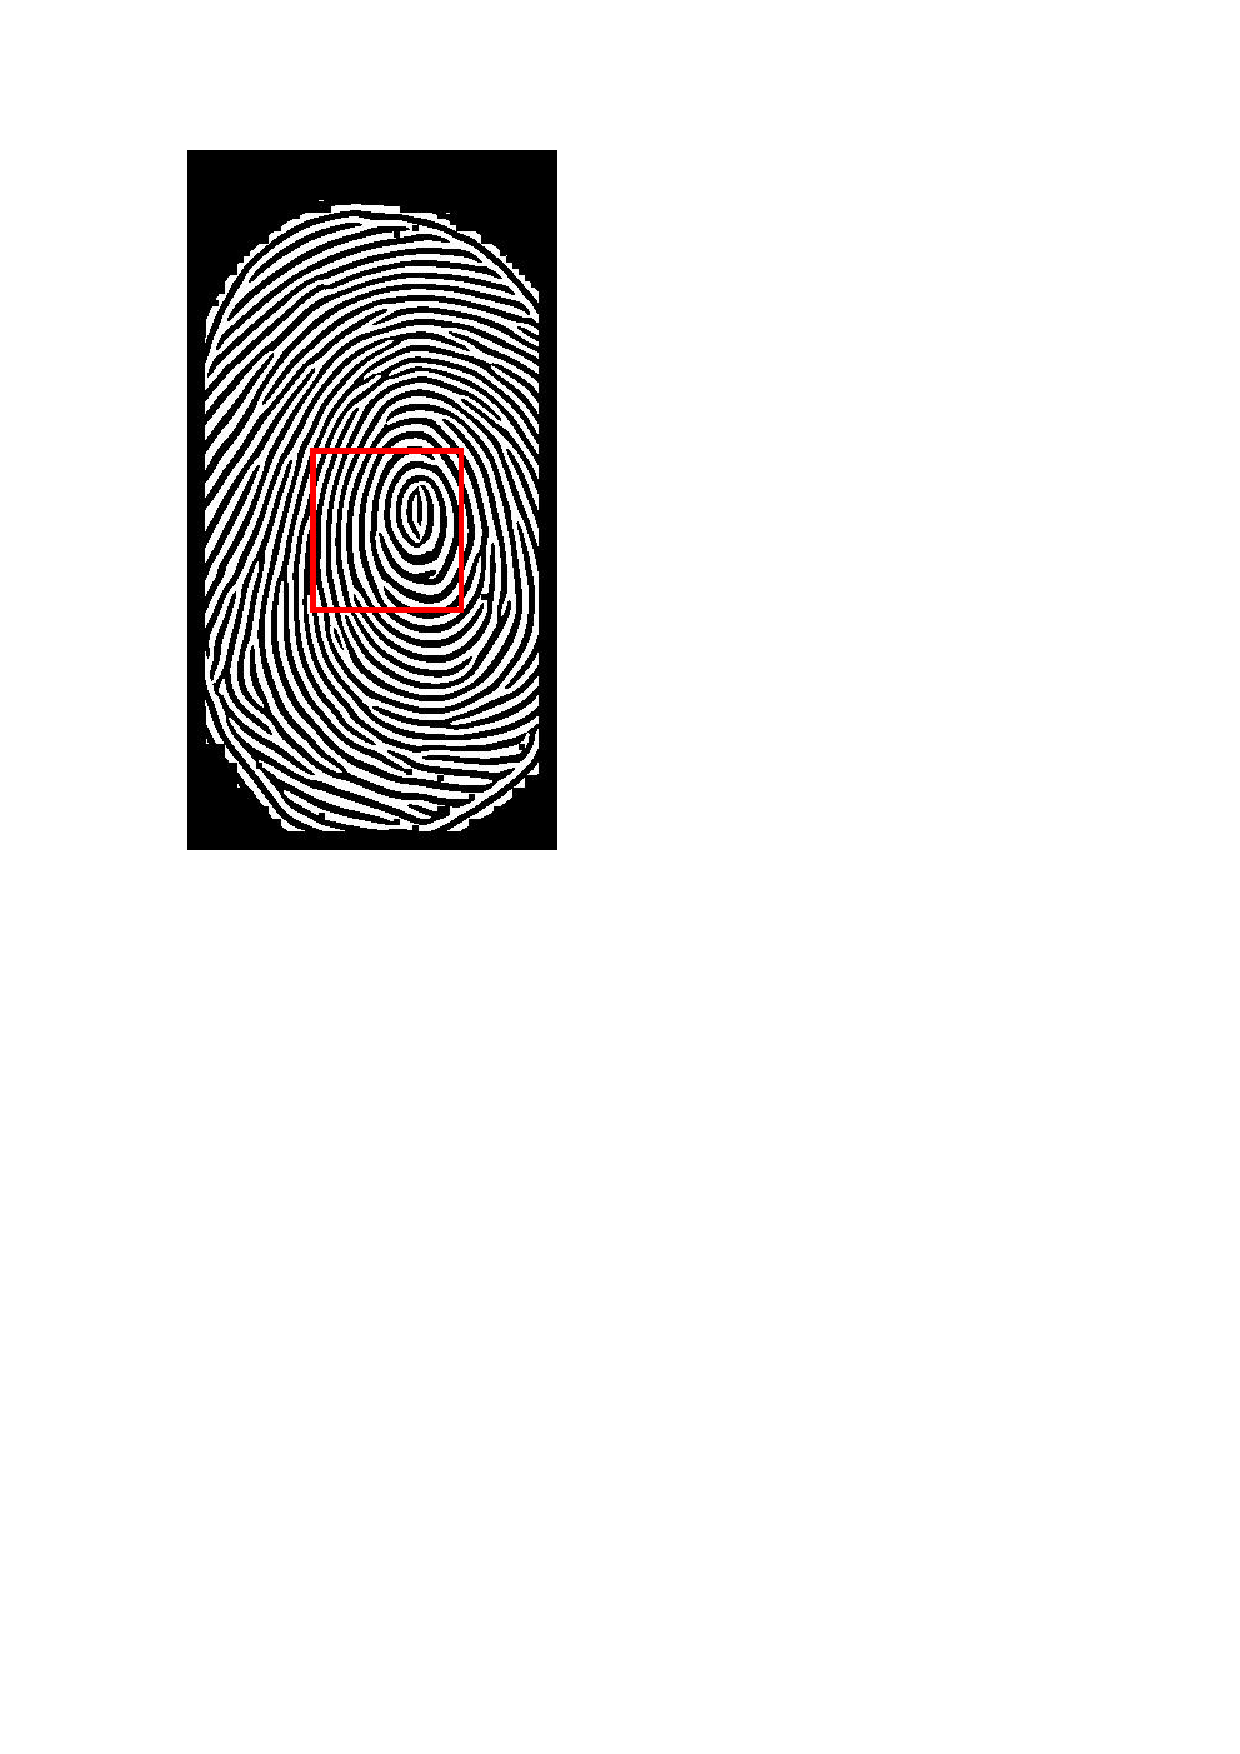
\includegraphics[width=0.57in]{images/glcm1.pdf}
		\label{fig:consistent1}} \subfigure[Scaled ROI of $r$.]{\centering
		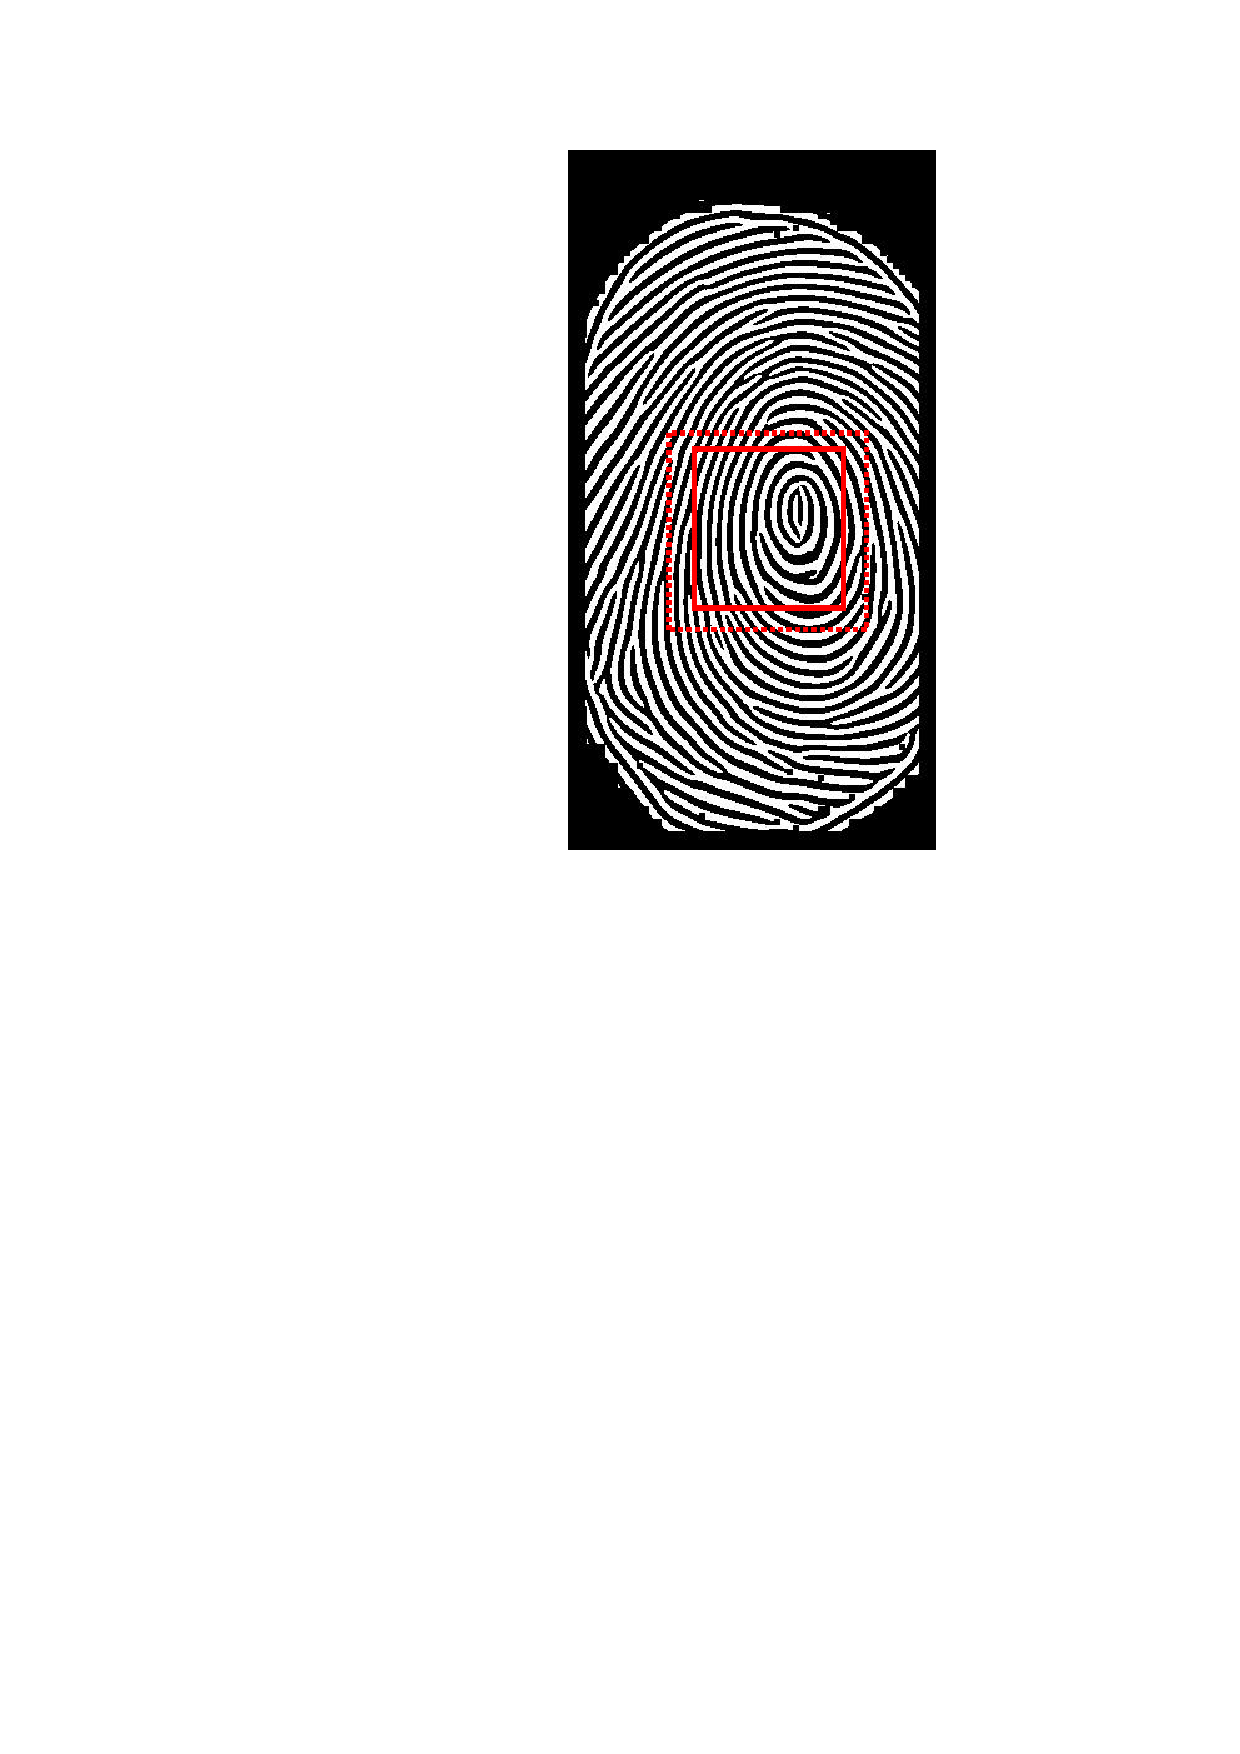
\includegraphics[width=0.55in]{images/glcm2.pdf}
		\label{fig:consistent2}} \subfigure[Consistent region.]{\centering
		\includegraphics[width=0.54in]{images/glcm3.pdf}
		\label{fig:consistent3}}
	\caption{Consistent region selection.}
	\label{fig:consistent}
	\vspace{-6mm}
\end{figure}

\par


\subsubsection{Feature extraction}
In most of the work reported in the literature, minutiae point-based features are
used in solving the verification and authentication problems~\cite{liu2017feature}. Such a feature is called a direct (also called
global) feature. However, the application of minutia features has the following
two shortcomings: (i) the minutiae feature extraction accuracy and (ii) the size
of the feature set, which depends on the number of minutiae points in an input
image. For example, in wet or crushed fingerprints, the number of extracted
minutiae is significantly lower, whereas, in dry fingerprints, false minutia
points are often observed due to the cuts in the ridges. For better
accuracy, it is advocated to follow indirect features and other features. Further, a combination
of multiple features of different nature can be a better alternative. This work
proposes a method of generating a hybrid feature vector combining the texture
features and indirect features. These features are extracted from the consistent
region of the fingerprint. The different feature extraction procedures are
described in the following sub-sections.

\subsubsubsection{Indirect feature vector extraction}
An indirect feature vector derived from a set of minutiae points is considered
for this work. Consider a fingerprint $f$; it consists of minutiae
features, which are points on the fingerprint, specifically ridge endings and
ridge bifurcations~\cite{liu2017feature}. A single minutia point has coordinates
$(x,y)$, and angle of orientation denoted by $\theta$~\cite{liu2017feature}.
Delaunay triangulation ~\cite{lee1980two} net is formed over the minutiae points in the
extracted region of interest. Delaunay triangulation~\cite{lee1980two} over a
given set of discrete points is the triangulation such that no point lies on the
circumference of any triangle. It maximizes the minimum angle among all angles
for all the triangles belonging to the triangulation. The triangulation gives a
stable structure that can be used to determine indirect features for a given
set of points. \par

First, the center of the region of interest (ROI) is approximated and
its distance is computed from the in-centers of all the triangles in the net.
Nearest neighboring triangles from the ROI's center are considered for further
processing. The indirect feature set for a particular fingerprint instance
obtained from the triangulation contains the concatenated information of
the relative area of each triangle, relative length (considering sides of
individual triangle), relative angle, relative in-center with respect to
individual
triangle, relative position and orientation as shown in Fig. \ref{fig:relative}.
Here, relative refers to normalized value with respect to the maximum value in
that particular set, for example $relative~ area~ =~ area~ of~ a~ \triangle~ /~
	max~ area ~of~ a~ \triangle~in~ triangulation$. The algorithm for relative
indirect feature vector generation is described as Algorithm~\ref{algo1}.\par
\begin{algorithm}
	\DontPrintSemicolon 
	\SetAlgoLined 
	\SetAlgoVlined 
	\SetNlSty{texttt}{(}{)}
	\LinesNumbered 
	\SetKwInOut{Input}{Input}
	\SetKwInOut{Output}{Output}
	\Input{ $f$ is a fingerprint.}
	\Output{feature vector $f_{v}$ of $f$ }
	%\BlankLine
	\caption{\textbf{Relative indirect feature vector generation}}
	\label{algo1}
	\textbf{Extract} the center of the ROI ($c$) $(x_{c},y_{c})$  \\
	\textbf{Extract} the minutiae features from the ROI. Let $i^{th}$ minutia in
	the ROI (having center $(x_{i},y_{i})$) be $(m_{i})$ \\
	\textbf{Form} $TR$ = delaunayTriangulation (on the minutiae points).\linebreak
	\textbf{Let} no. of triangles in TR = $t$
	\linebreak
	\textbf{Let} in-center of $j^{th}$ triangle in $TR$ be $(x_{j},y_{j})$  \\
	\For{i=j to t}{ $d\left( c,t_{i}\right)   = \sqrt { \left(
				x_{c}-x_{i}\right)^2 + \left( y_{c}-y_{i}\right)^2 } 	$
	
	} \textbf{Select} $k$ nearest triangles from the center of ROI ($c$)
	$(x_{c},y_{c})$  \linebreak
	Let the term \textbf{relative} be denoted by $\textbf{r}$\\
	\For{i=1 to k}{ r\_area($\triangle z_{i}$) = area($\triangle z_{i}$) /
		max(area($\forall$ $\triangle \in$ TR))\\

		r\_length\_of\_sides($\triangle z_{i}$) = length\_of\_sides($\triangle
		z_{i}$) / max(length\_of\_sides($\forall$ $\triangle \in$ TR))\\

		r\_angles\_b/w\_sides($\triangle z_{i}$) = angles\_b/w\_sides($\triangle
		z_{i}$) / max(angles\_b/w\_sides($\forall$ $\triangle \in$ TR))\\

		r\_incenter($\triangle z_{i}$) = incenter($\triangle z_{i}$) /
		max(incenter($\forall$ $\triangle \in$ TR))\\ }

	\For{i=1 to 10}{
		\tcc{Ten consistent minutia selected in the consistent region.}
		r\_position\_value($m_{i}$) = position($m_{i}$) /
		max(position\_value($\forall$ $m_{i}~\in~ m$))\\ r\_orientation($m_{i}$)
		= orientation($m_{i}$) / max(orientation($\forall$ $m_{i}~\in~ m$))\\ }
	\textbf{ feature vector($f_{v}$)}=   [r\_area($\forall$ $\triangle \in$
	TR) $\mathbin\Vert$ r\_length\_of\_sides($\forall$ $\triangle{i} \in$
	TR) $\mathbin\Vert$ r\_angles\_b/w\_sides($\forall$ $\triangle \in$ TR)
	$\mathbin\Vert$ r\_incenter($\forall \triangle \in$ TR) $\mathbin\Vert$
	r\_position($\forall$ $m_{i}~\in~ m$) $\mathbin\Vert$
	r\_orientation($\forall$ $m_{i}~ \in ~m$) ]
\end{algorithm}
\begin{figure}[!ht]
	\centering
	\subfigure[Delaunay triangular net from a set of minutia points.]{
		\centering
		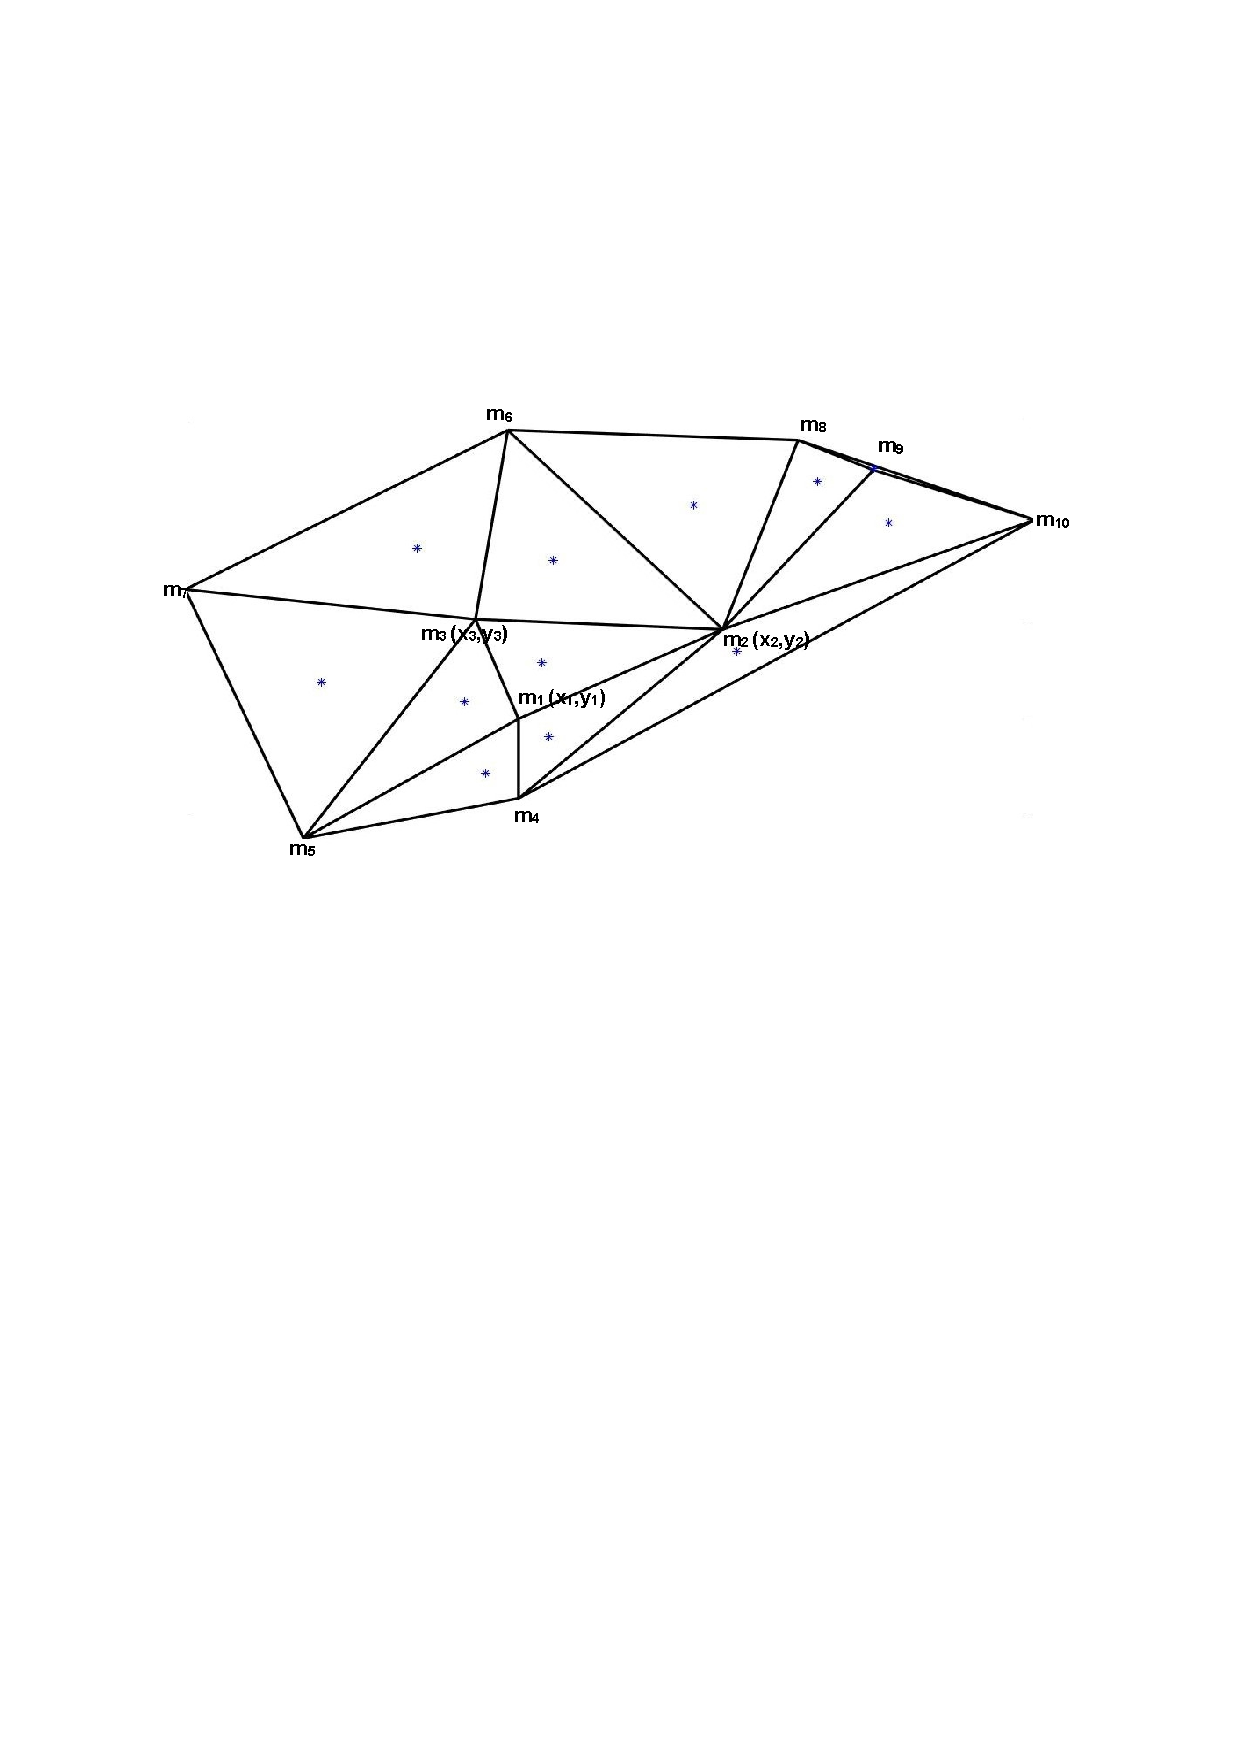
\includegraphics[width=2.8in]{images/Diagramsdelunay1.pdf}
		\label{fig:realtive1}} \subfigure[Indirect feature extraction from a
		triangle.]{\centering
		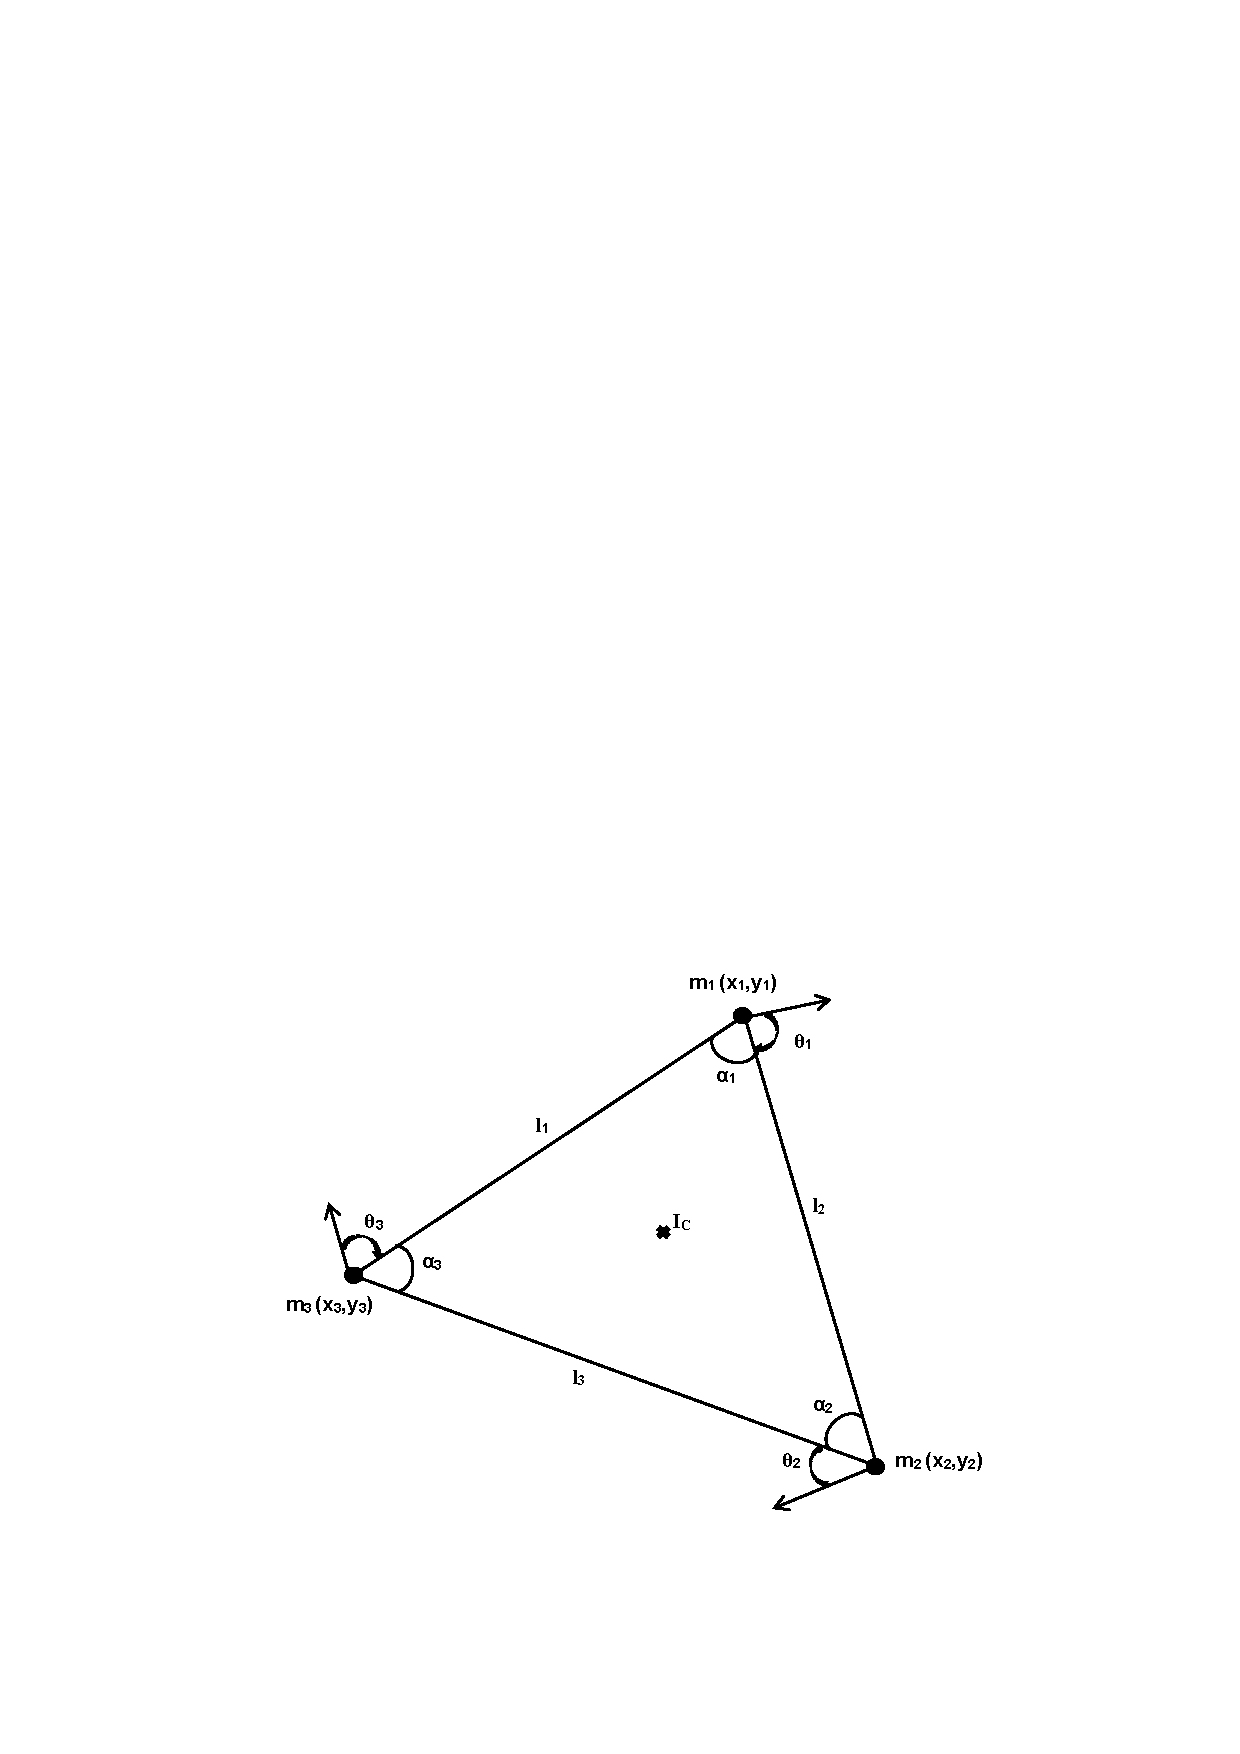
\includegraphics[width=2.0in]{images/Diagramsdelunay2.pdf}
		\label{fig:realtive2}}
	\caption{An example of Delaunay triangulation-based indirect feature generation.}
	\label{fig:relative}
	\vspace{-6mm}
\end{figure}

\par

\subsubsubsection{Texture-based feature extraction}
"Texture" is a characteristic item in any fingerprint image. ~Local texture
descriptors are invariant to illumination changes, are discriminative, and
resistant to noise and image blurring. The computational complexity of finding
texture descriptors is low compared to other feature extractions~\cite{li2019learning}.
The proposed work uses Hilbert curve-based descriptor (HCBD)  \cite{Ebrahim2009hcbd}, gray code-based
descriptor (GCBD) \cite{Zhao2008gcbd}, Local ternary pattern (LTP) \cite{tan2010enhanced} and Median
ternary pattern (MTP)~\cite{bashar2014robust} to extract texture features from
the fingerprint's consistent region.

\par

\noindent \textbf{Hilbert curve and Gray code-based descriptors:}
Hilbert curve and gray code curve are space-filling curves that are used to preserve the
mapping of multidimensional points in a one-dimensional space. Two descriptors,
namely  Hilbert curve-based descriptor
(HCBD) and Gray code-based descriptor (GCBD) are followed in this work. These
descriptors are robust and efficient, insensitive to illumination and
intensities, and rotation, scaling and shift invariant. These descriptors, unlike
the traditional descriptors, consider a window of $4 \times 4$.  Let $I$,
$P_{s}^{(i,j)}$ be the starting pixel of a  $4 \times 4$  window having gray
value $I_{1}^{(i,j)}$ in a gray-scale image. The $n^{th}$ neighbor of
$P_{s}^{(i,j)}$ is denoted as $P_{n}^{(i,j)}$ in Hilbert and gray code pattern
traversal, where $n$ is a positive integer ($n \in [1,N]$)  and $N=16$. The
Hilbert curve based operator is defined in Equation (\ref{eq17}), (\ref{eq18})
and (\ref{eq19}).

\begin{equation}\label{eq17}
	HCBD_{l}(i,j)=\sum_{n=2}^{N/2}sign(I_{n}^{(i,j)}-I_{n-1}^{(i,j)})\times 2^{n-1}
\end{equation}
\begin{equation}\label{eq18}
	HCBD_{u}(i,j)=\sum_{n=N/2+2}^{N}sign(I_{n}^{(i,j)}-I_{n-1}^{(i,j)})\times 2^{n-1}
\end{equation}
%$HCBD=$ \begin{equation}\label{eq19} \begin{split} \\\left\{\begin{matrix}
%[HCBD_{l} \oplus  HCBD_{u} || 0] ,& if
%sign(I_{N/2+1}^{(i,j)}-I_{N/2}^{(i,j)})=1\\ [HCBD_{l} \oplus  HCBD_{u} || 1], &
%if  sign(I_{N/2+1}^{(i,j)}-I_{N/2}^{(i,j)})=-1 \end{matrix}\right. \end{split}
%\end{equation}
\begin{equation}\label{eq19}
	HCBD=\left\{\begin{matrix}
		[HCBD_{l} \oplus  HCBD_{u} || 0] , & if sign(I_{N/2+1}^{(i,j)}-I_{N/2}^{(i,j)})=1   \\
		[HCBD_{l} \oplus  HCBD_{u} || 1],  & if  sign(I_{N/2+1}^{(i,j)}-I_{N/2}^{(i,j)})=-1
	\end{matrix}\right.
\end{equation}
where $\oplus$ is $XOR$ operator and $||$ is the concatenation operator. The
HCBD operator is illustrated in Fig.\ref{HCBD1}.

\begin{figure}[!ht]
	\centering
	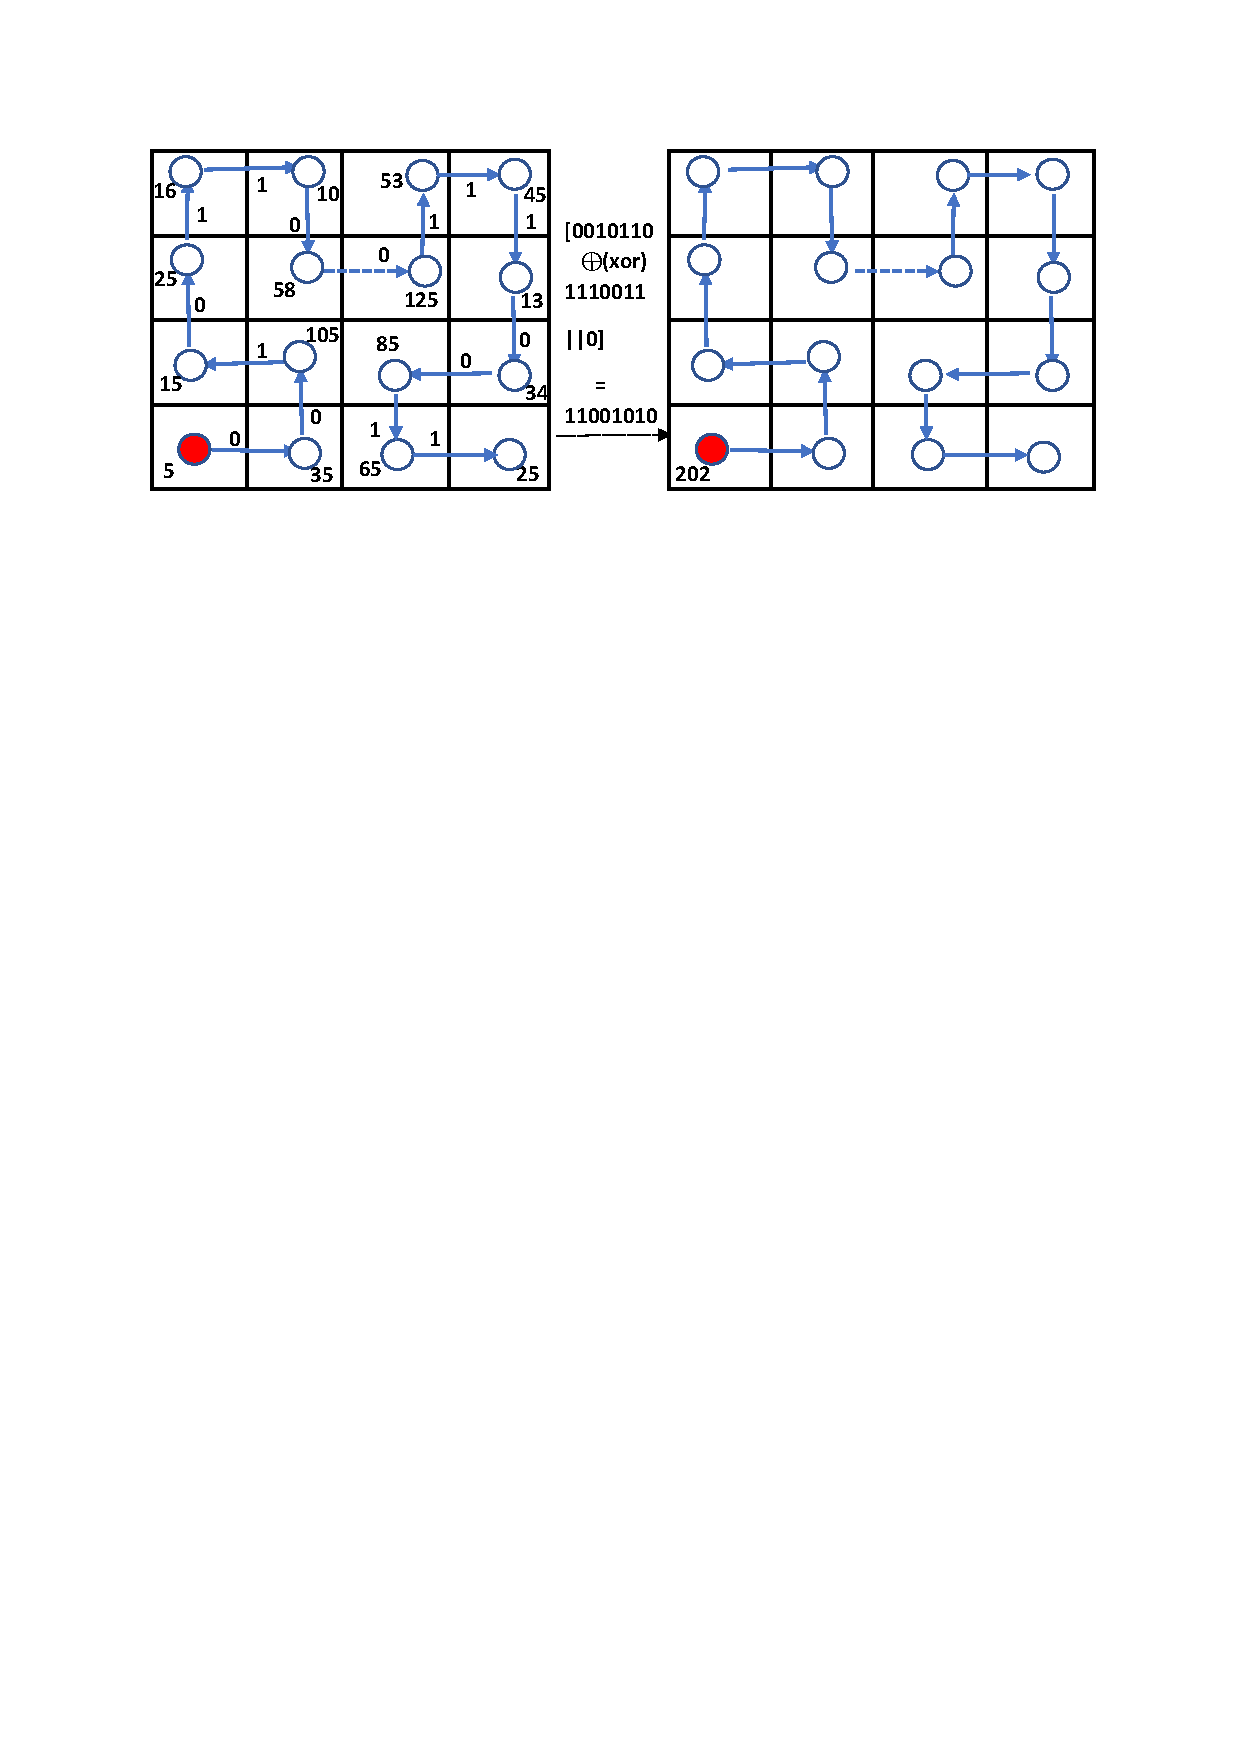
\includegraphics[width=2.0in]{images/hcbd.pdf}
	\caption{Illustration of HCBD operator.}
	\label{HCBD1}
	\vspace{-4mm}
\end{figure}

\par

Similarly, gray code curve-based operator is defined in Equation (\ref{eq20}),
(\ref{eq21}) and (\ref{eq22}).
\begin{equation}\label{eq20}
	GCBD_{l}(i,j)=\sum_{n=2}^{N/2}sign(I_{n}^{(i,j)}-I_{n-1}^{(i,j)})\times 2^{n-1}
\end{equation}
\begin{equation}\label{eq21}
	GCBD_{u}(i,j)=\sum_{n=N/2+2}^{N}sign(I_{n}^{(i,j)}-I_{n-1}^{(i,j)})\times 2^{n-1}
\end{equation}
%$GCBD=$ \begin{equation}\label{eq22} \begin{split} \\\left\{\begin{matrix}
%[GCBD_{l} \oplus  GCBD_{u} || 0] ,& if
%sign(I_{N/2+1}^{(i,j)}-I_{N/2}^{(i,j)})=1\\ [GCBD_{l} \oplus  GCBD_{u} || 1], &
%if  sign(I_{N/2+1}^{(i,j)}-I_{N/2}^{(i,j)})=-1 \end{matrix}\right. \end{split}
%\end{equation}
\begin{equation}\label{eq22}
	GCBD=
	\left\{\begin{matrix}
		[GCBD_{l} \oplus  GCBD_{u} || 0] , & if sign(I_{N/2+1}^{(i,j)}-I_{N/2}^{(i,j)})=1   \\
		[GCBD_{l} \oplus  GCBD_{u} || 1],  & if  sign(I_{N/2+1}^{(i,j)}-I_{N/2}^{(i,j)})=-1
	\end{matrix}\right.
	%\end{split}
\end{equation}
where $\oplus$ is $XOR$ operator and $||$ is the concatenation operator. The
GCBD operator is illustrated in Fig.\ref{GCBD1}.

\begin{figure}[!ht]
	\centering
	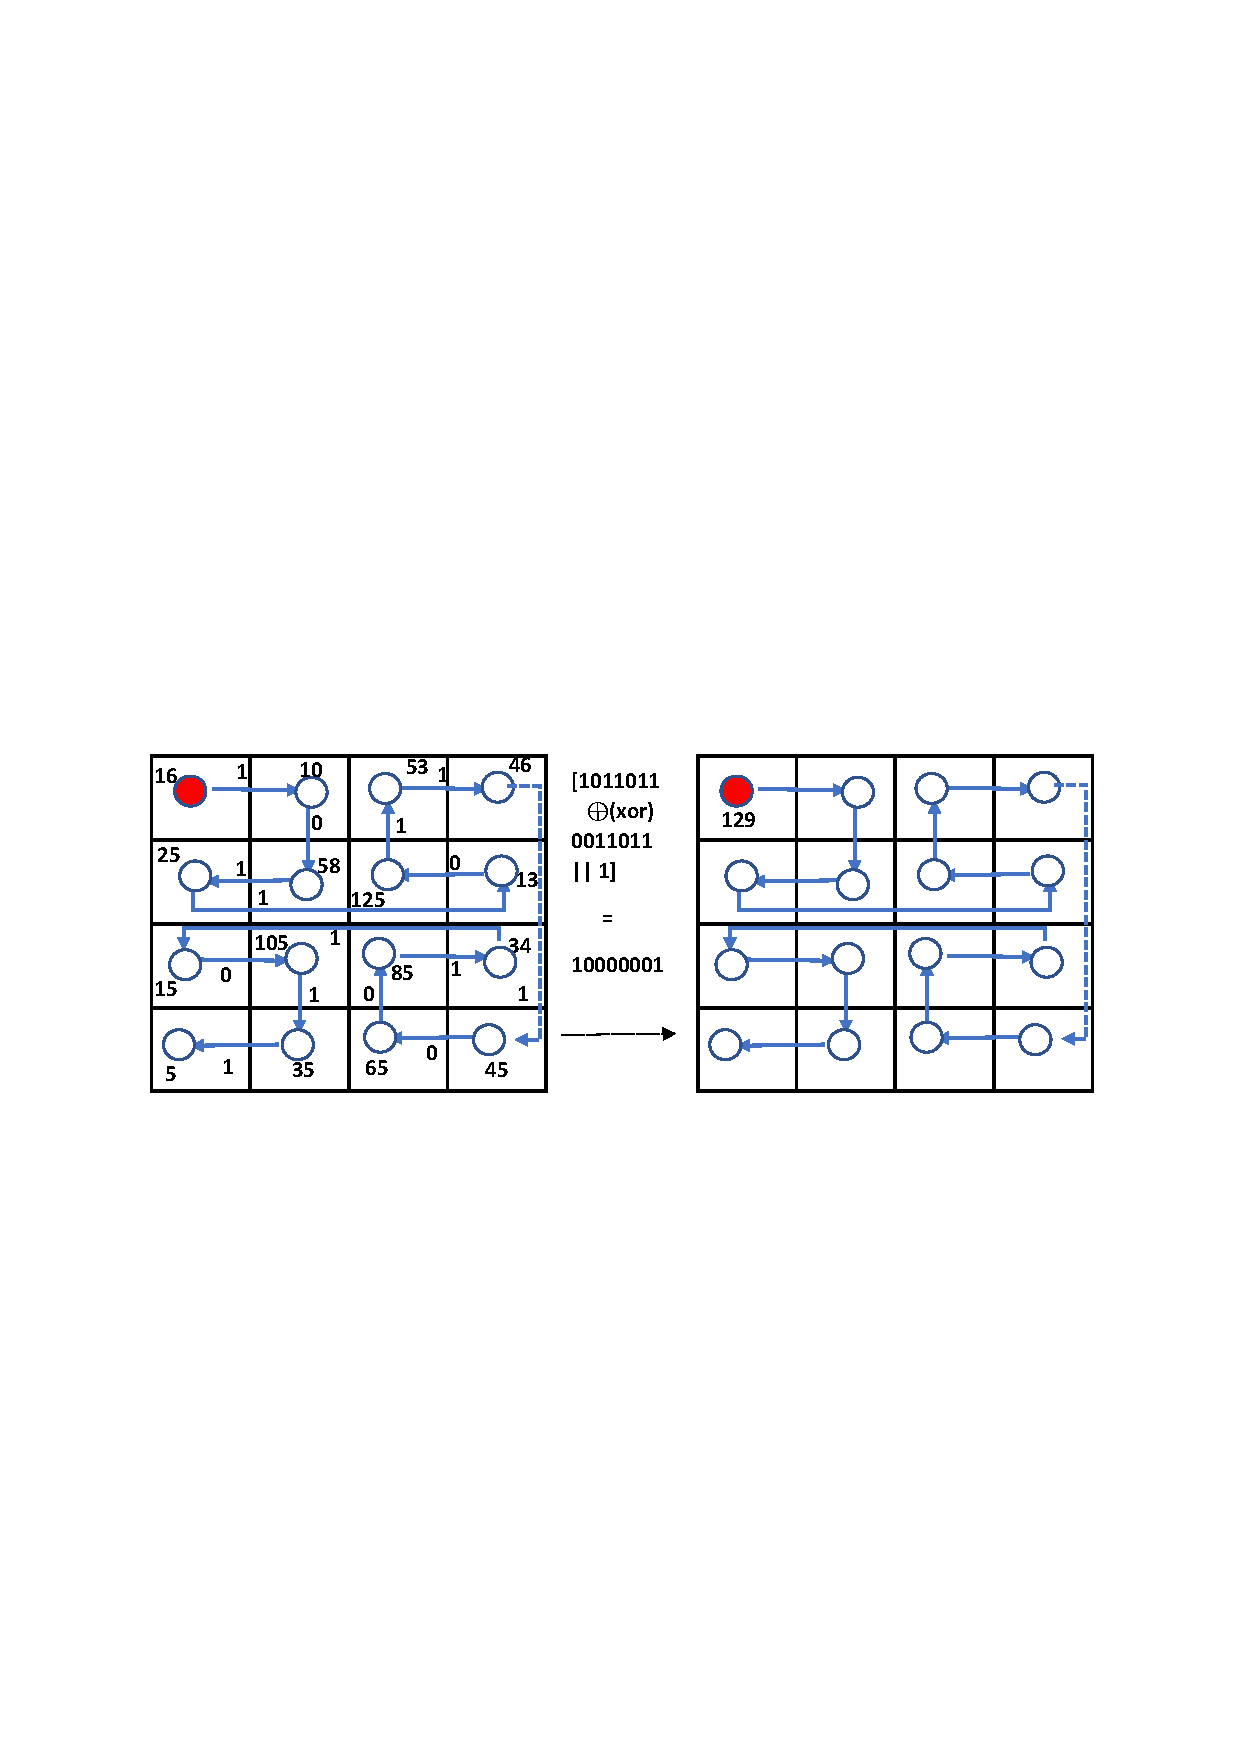
\includegraphics[width=2.0in]{images/gcbd.pdf}
	\caption{Illustration of GCBD operator.}
	\label{GCBD1}
	% \vspace{-6mm}
\end{figure}

\noindent \textbf{Local Ternary Pattern:} Tan and Triggs~\cite{tan2010enhanced}
presented a new texture operator having three value codes $(-1,0,1)$ unlike two
value codes in the local binary pattern. This operator is more robust towards noise.
The mathematical expression of an LTP is given below.

\begin{equation}
	LTP_{P,R}=\sum_{p=0}^{P-1}2^{P}s(i_{p}-i_{c})
\end{equation}

where $i_{c}$ denotes the gray values of the center
pixel and $i_{p}$ $(p = 0,..., P-1)$ denotes the gray value of a neighbor pixel
on a circle of radius $R$. $P$ denotes the number of neighbors. Bilinear
interpolation estimation is used to estimate the neighbors that do not lie exactly in the center
of the pixels.

\begin{equation}
	s(u)=\left\{\begin{matrix}
		1  & u \geq t   \\
		0  & -t < u < t \\
		-1 & u < -t
	\end{matrix}\right.
\end{equation}

where $t$ is a threshold value. Now, the LTP is the concatenation of histograms
obtained from both $LTP_{u}$, $LTP_{l}$, where $LTP=LTP_{u} || LTP_{l}$ as shown
in Fig. \ref{fig:ltp}. A single LTP feature descriptor is of size 512.\\

\begin{figure}[!ht]
	\centering
	\subfigure[Orginal image block of size $3 \times 3$.]{
		\centering
		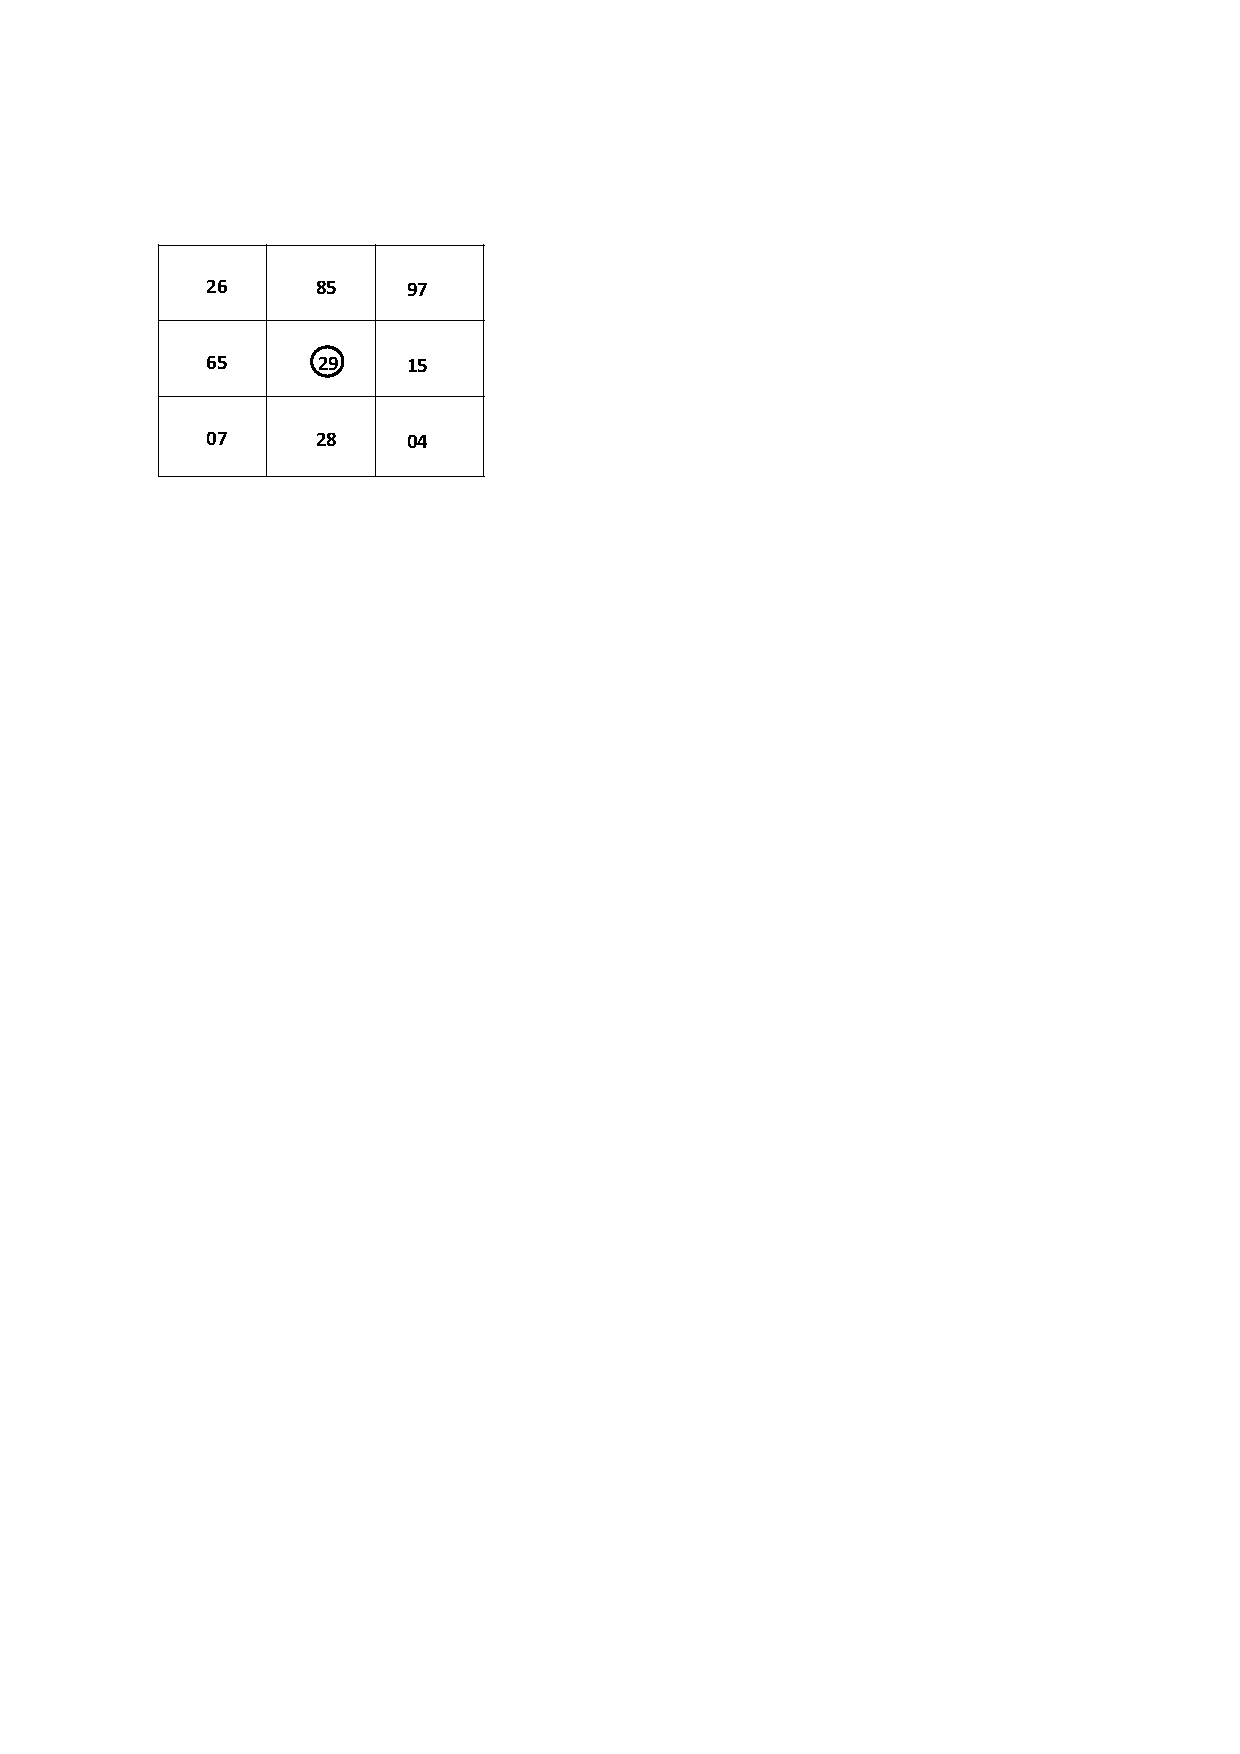
\includegraphics[width=1in]{images/LTP1.pdf}
		\label{fig:ltp1}} \subfigure[LTP code $1011(-1)(-1)0(-1)$ with center
		pixel value $29$ and threshold $t=5$.]{\centering
		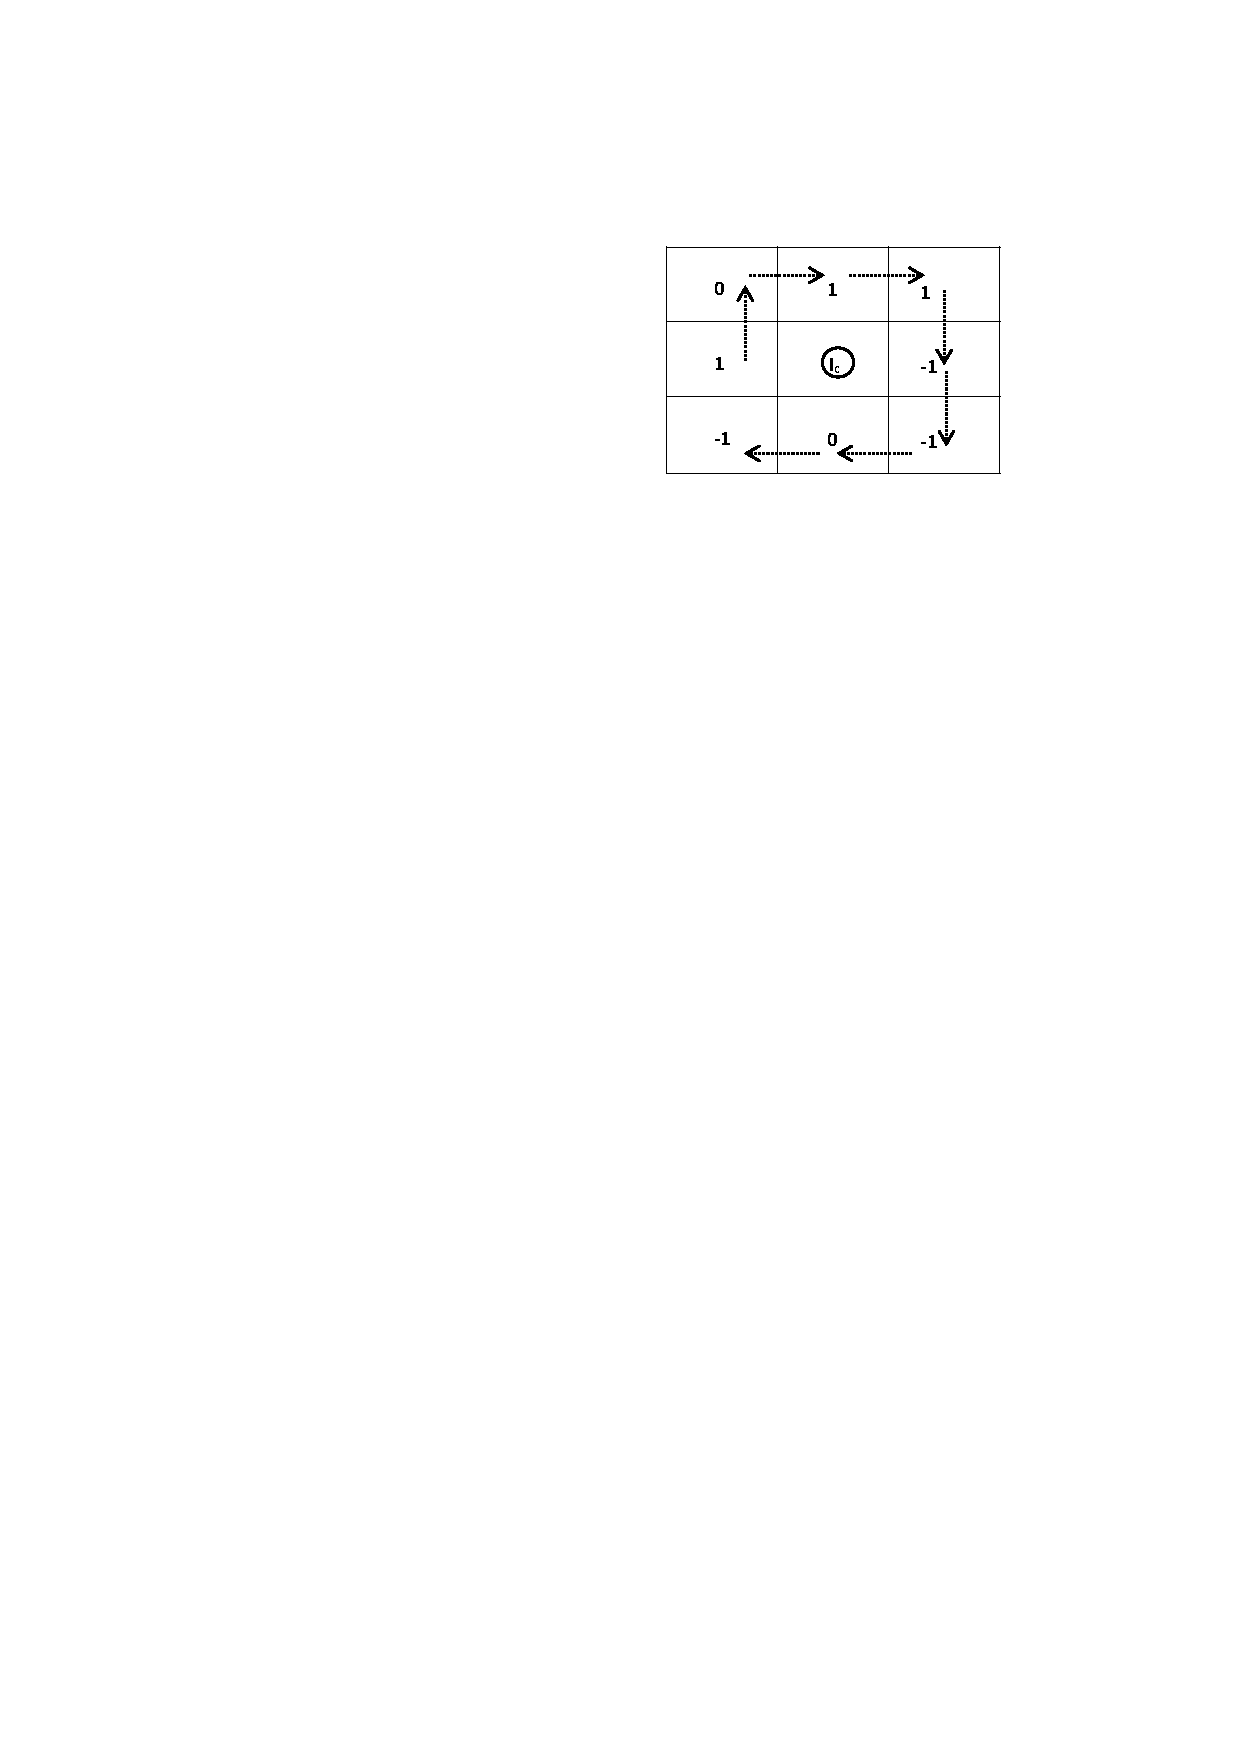
\includegraphics[width=1in]{images/LTP2.pdf}
		\label{fig:ltp2}}
	\subfigure[$LTP_{u}$ code $10110000$ and $I_{c}$ is assigned to
		176.]{\centering
		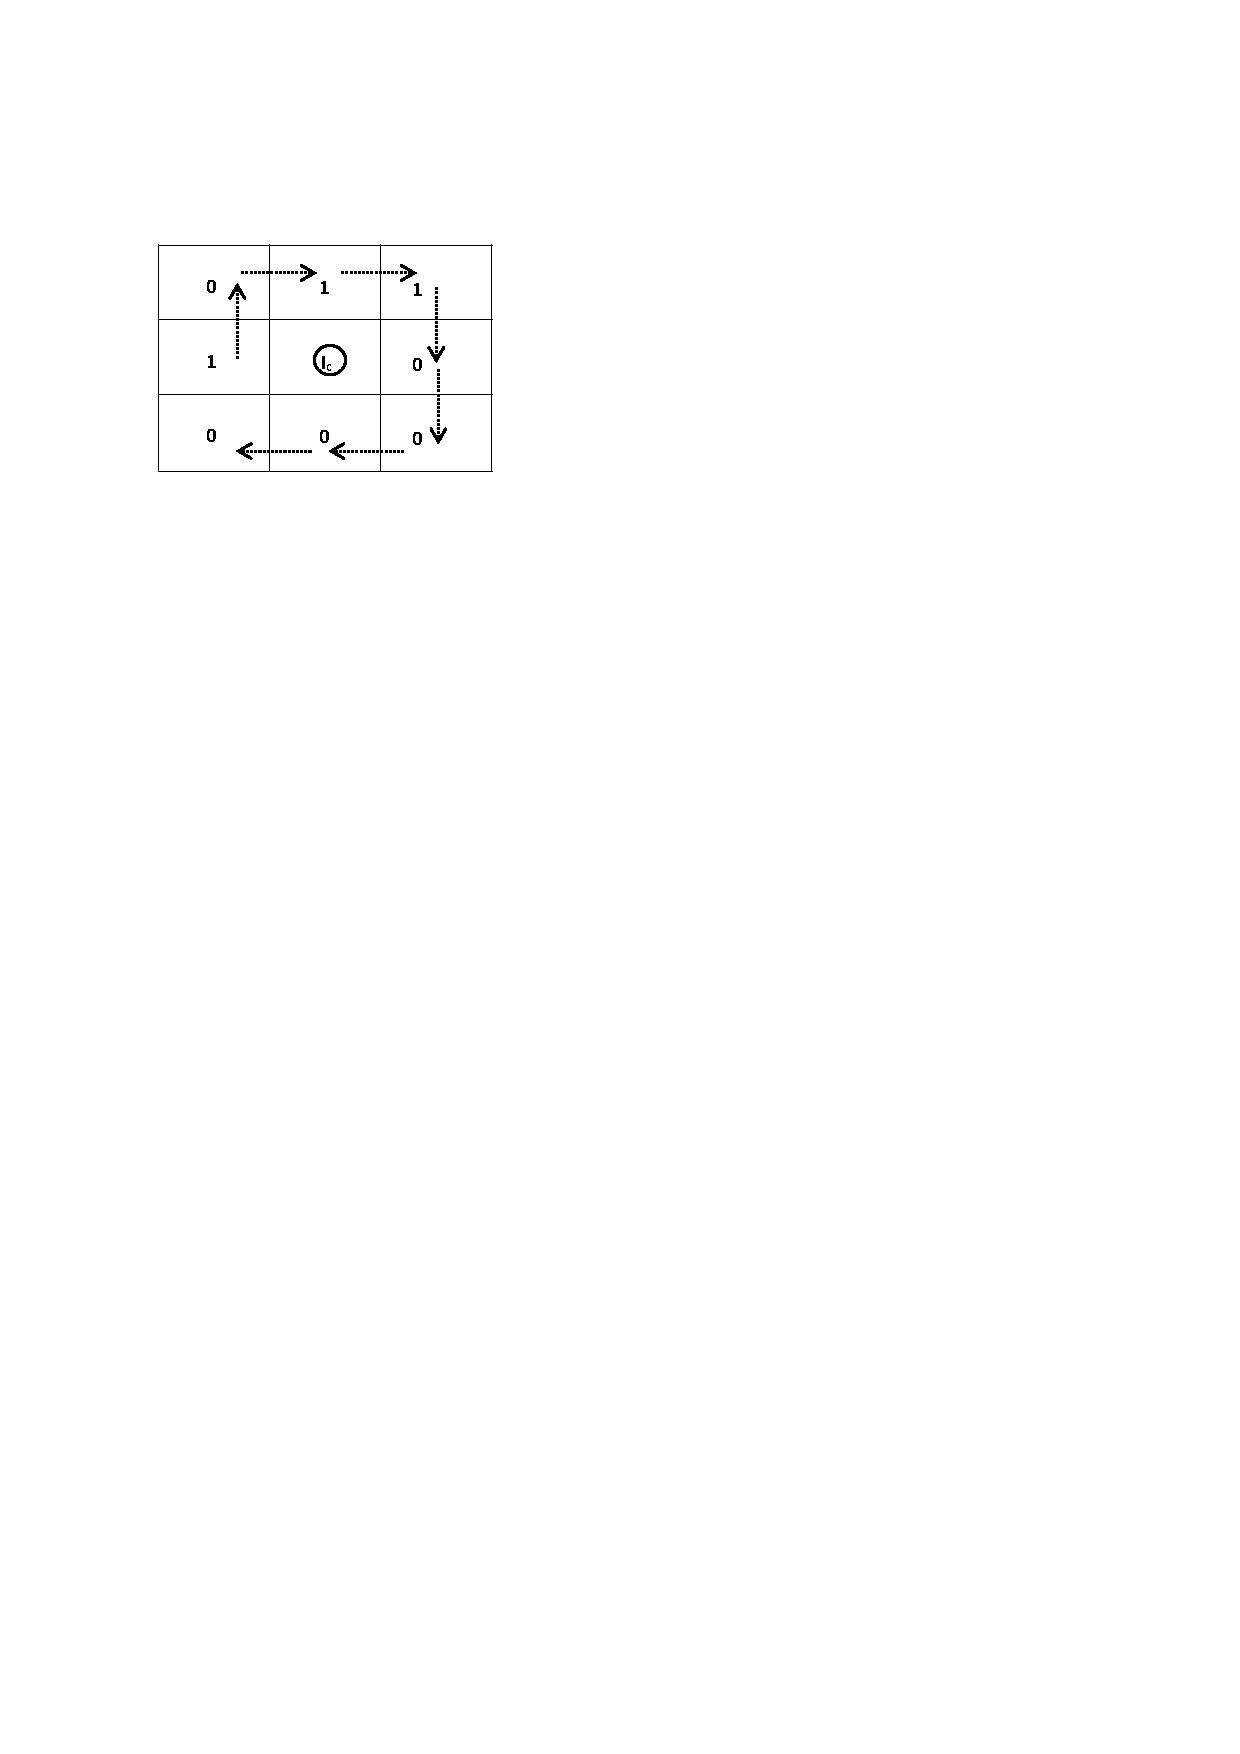
\includegraphics[width=1in]{images/LTP3.pdf}
		\label{fig:ltp3}} \subfigure[$LTP_{l}$ code $00001101$ and $I_{c}$ is
		assigned to 13.]{\centering
		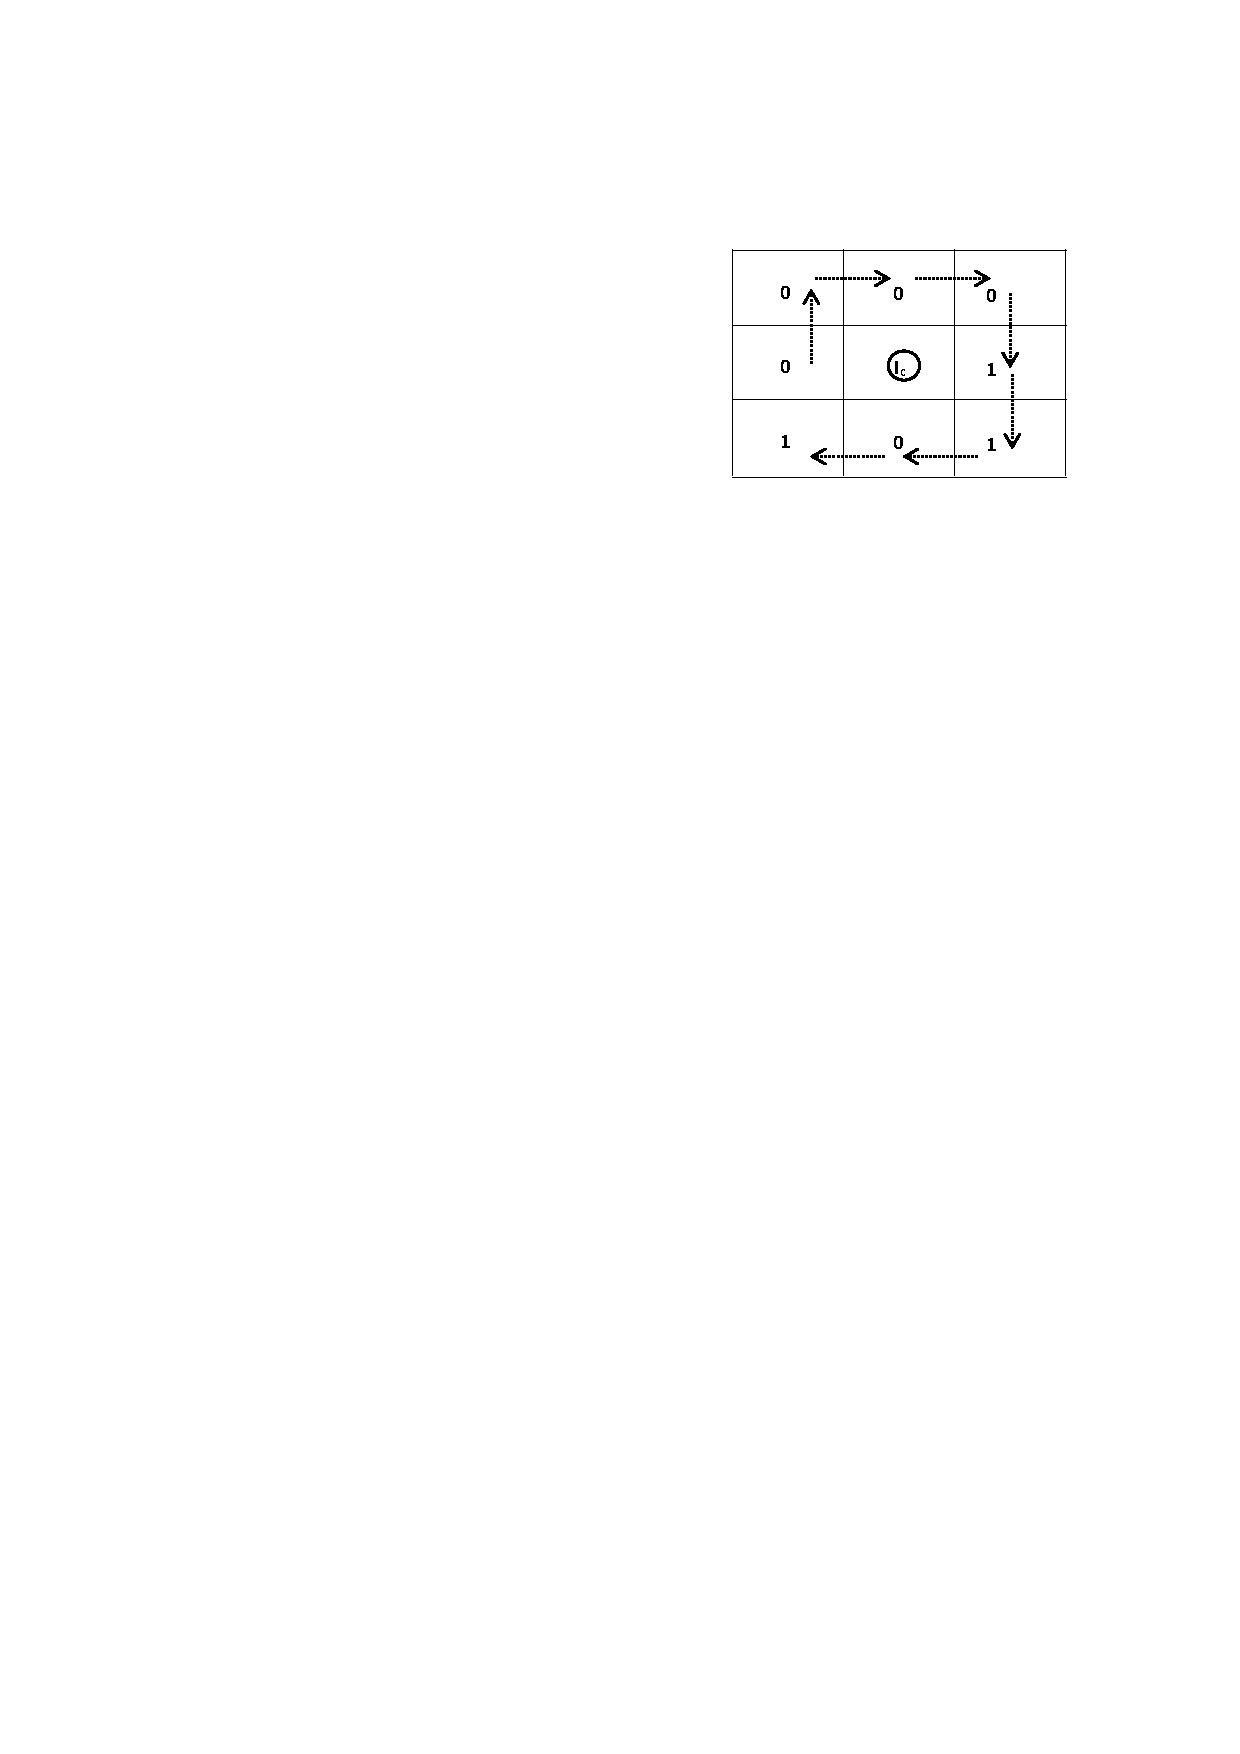
\includegraphics[width=1in]{images/LTP4.pdf}
		\label{fig:ltp4}}
	\caption{Illustration of LTP operator.}
	\label{fig:ltp}
	\vspace{-4mm}
\end{figure}

\noindent \textbf{Median Ternary Pattern:} Median filters perform well in the
presence of noise. Therefore, a method that exploits the median can more
accurately extract the information from any texture than the local binary patterns.
Bashar et al. \cite{bashar2014robust} proposed Median Ternary Pattern(MTP) that
combines the advantages of median and quantization of the pixel's gray scale
value. The MTP code is derived using the following equations:

\begin{equation}
	s^{\prime}(u)=\left\{\begin{matrix}
		1  & u \geq m_{c}+t       \\
		0  & m_{c}-t < u <m_{c}+t \\
		-1 & u < m_{c}-t
	\end{matrix}\right.
\end{equation}

Here, $u$ is a neighbor gray level, $m_{c}$ is the local median, and $t$ is a
user specified threshold. The feature code length is $3^{8}$. To reduce the
feature vector to $2 \times 2 ^{8}$, MTP is further split into $MTP_{u}$ and
$MTP_{l}$ as shown in Fig. \ref{fig:mtp}. Final MTP is concatenation of both
$MTP_{u}$ and $MTP_{l}$. The $MTP_{u}$ can be derived as follows.

\begin{equation}
	MTP_{u}=\sum_{p=0}^{7}f_{u}(s^{\prime}(i_{p})) \times 2^{P},
	f_{u}(x)=\left\{\begin{matrix}
		1 & x =1      \\
		0 & otherwise \\
	\end{matrix}\right.
\end{equation}

$MTP_{l}$ is derived using the following equation:

\begin{equation}
	MTP_{l}=\sum_{p=0}^{7}f_{l}(s^{\prime}(i_{p})) \times 2^{P},
	f_{l}(x)=\left\{\begin{matrix}
		1 & x=-1      \\
		0 & otherwise \\
	\end{matrix}\right.
\end{equation}

\begin{figure}[!ht]
	\centering
	\subfigure[Orginal image block of size $3 \times 3$.]{
		\centering
		\includegraphics[width=1in]{images/MTP1.pdf}
		\label{fig:mtp1}} \subfigure[MTP code $(-1)(-1)10000$ with median $86$
		and threshold $t=10$.]{\centering
		\includegraphics[width=1in]{images/MTP2.pdf}
		\label{fig:mtp2}} \subfigure[$MTP_{u}$ code $0010000$ and $I_{c}$ is
		assigned to 16.]{\centering
		\includegraphics[width=1in]{images/MTP3.pdf}
		\label{fig:mtp3}} \subfigure[$MTP_{l}$ code $1100000$ and $I_{c}$ is
		assigned to 96.]{\centering
		\includegraphics[width=1in]{images/MTP4.pdf}
		\label{fig:mtp4}}
	\caption{Illustration of MTP operator.}
	\label{fig:mtp}
	\vspace{-4mm}
\end{figure}
%\begin{figure}[!t] \centering \subfigure[Orginal image block of size \\$3
%   \times 3$.]{ \centering \includegraphics[width=1.5in]{MTP1.pdf}
%   \label{fig:mtp1}} \subfigure[MTP code $(-1)(-1)10000$ with median $86$ and
%   threshold $t=10$.]{\centering \includegraphics[width=1.5in]{MTP2.pdf}
%   \label{fig:mtp2}} \subfigure[$MTP_{u}$ code $0010000$ and \\ $I_{c}$ is
%   assigned to 16.]{\centering \includegraphics[width=1.5in]{MTP3.pdf}
%   \label{fig:mtp3}} \subfigure[$MTP_{l}$ code $1100000$ and $I_{c}$ is
%   assigned to 96.]{\centering \includegraphics[width=1.5in]{MTP4.pdf}
%   \label{fig:mtp4}} \caption{Illustration of MTP operator.} \label{fig:mtp}
%   \end{figure}\\
\noindent \textbf{Texture based feature extraction methodology:} The proposed
texture-based method combines the features from HCBD (256 bits), GCBD (256
bits), LTP (512 bits) and MTP (512 bits). The steps are as follows:
\begin{itemize}
	\item \textbf{ Step-1:} Around each minutiae point in the consistent region,
	      HCBD features $f_{hcbd}$, GCBD features $f_{gcbd}$, LTP features
	      $f_{ltp}$, and MTP features $f_{mtp}$ are extracted with a window of
	      size $w \times w$.
	\item \textbf{ Step-2:} All $f_{hcbd}$,$f_{gcbd}$,$f_{ltp}$,$f_{mtp}$
	      features from all minutia patches are combined and these texture
	      features are defined by building a histogram as $F_{hcbd}$,$F_{gcbd}$,$F_{ltp}$,$F_{mtp}$.
	      % \item \textbf{ Step-3:} Combine all $f_{gcbd}$ features from all minutia
	      %       patches and then these texture features are defined by building a
	      %       histogram $F_{gcbd}$.
	      % \item \textbf{ Step-4:} Combine all $f_{ltp}$ features from all minutia
	      %       patches and then these texture features are defined by building a
	      %       histogram $F_{ltp}$.
	      % \item \textbf{ Step-5:} Combine all $f_{mtp}$ features from all minutia
	      %       patches and then these texture features are defined by building a
	      %       histogram $F_{mtp}$.
	\item \textbf{ Step-3:} Normalized feature vector $F_{T1}$ is obtained by
	      applying z-score normalization on the concatenated features $F_{hcbd}$,
	      $F_{gcbd}$ and $F_{ltp}$ (not including $F_{mtp}$).
	      \subitem  $F_{T1}$ = z-score$(F_{hcbd}||
		      F_{gcbd} ||F_{ltp})$.
	\item \textbf{ Step-4:} Normalized feature vector $F_{T2}$ is obtained
	      applying z-score normalization on all the concatenated features $F_{hcbd}$,
	      $F_{gcbd}$, $F_{ltp}$ and $F_{mtp} $.
	      \subitem  $F_{T2}$ = z-score$(F_{hcbd}|| F_{gcbd} ||F_{ltp}||F_{mtp})$.\\
	      Here, z-score, denoted by z, is $z = (x - \mu) / (\sigma)$,
	      where $\mu$ is the mean value of the features and $\sigma$ is the
	      standard deviation of the features.
\end{itemize}
Furthermore, normalized relative minutia feature vectors and texture-based
feature vectors are fused to obtain a hybrid feature vector($F_{h}$).



\subsubsection{Prominent feature selection}
In the method discussed so far, a combination of features~($F_{h}$) of a
fingerprint image data is considered. An initial investigation revealed that all
feature vector components do not equally contribute to a distinct
feature vector generation. Thus the need to select the prominent feature
arises. ~To select the prominent features from the
combined feature vector, a genetic algorithm-based feature selection technique
is proposed.

\par

Genetic algorithm(GA)~\cite{chiesa2020gars,alirezazadeh2015genetic} is a
powerful optimization technique to select the best subset of features from a
feature vector. The combined feature vector obtained from the fingerprint image
is optimized through GA. This optimized vector, or prominent feature set, is
smaller in size but contains more relevant information. This vector is less prone
to noise and has distinct information. In this work, different GA parameters
are chosen based on an empirical experiment and the optimized values of
different GA parameters are shown in
Table \ref{table:GA}. The experimental procedure for the procedure is as follows.

\begin{itemize}
	\item \textbf{Step-1:} An initial population size of 10 is generated. The
	      length of each feature vector ($F_{h}$), henceforth referred as chromosome, is $L$.
	\item \textbf{Step-2:} The fitness value or accuracy of each chromosome is
	      determined. For the proposed method, KNN classifier is used to
	      evaluate this parameter by dividing the total feature set into 2
	      parts, namely training set and testing set.
	\item \textbf{Step-3:} Rank-based selection method is used to find the
	      fittest chromosome for mating.
	\item \textbf{Step-4:} A 2-point crossover is applied on $80 \% $ of the
	      selected chromosome, and the rest  $20 \%$  is added through elitism. This
	      process generates new offsprings.
	\item \textbf{Step-5:} Mutations in the chromosome is performed with
	      probability 0.01 to generate a new population.
	\item \textbf{Step-6:} \textbf{Step-2} to \textbf{Step-5} is performed until number of generations reach 100.
\end{itemize}

\begin{table}[!ht]
	\caption{GA constraints information.}
	\label{table:GA}
	\begin{center}
		%	\resizebox{\columnwidth}{!}{
		\begin{tabular}{|l|c|}
			\hline
			GA parameters           & Value \\ \hline
			Initial population size & 10    \\
			%				Each chromosome size & \textbf{$0.6$  $ \times$
			%				length of original feature vector($F_{h}$)}
			%				\\
			No of generation        & 100   \\ Crossover probability & 0.80 \\
			Mutation probability    & 0.01  \\ \hline
		\end{tabular}%}
	\end{center}

\end{table}
By applying GA on the combined feature set $F_{h}$, the prominent features are obtained.

% Let the length of each feature vector be $L_{g}$.
% where  $L_{g} \in [72,324,720,1024]$ with respect to different feature
% combination. 
% \begin{figure}[!t] 
% 	\centering 
% 	\includegraphics[width=5in]{ga.pdf}
% 	\caption{GA process} 
% 	\label{ga} 
% \end{figure}

\subsubsection{Discriminant feature vector generation}
The indirect feature vector should be distinct, that is,
the intra-class fingerprint feature vectors must be distinguishable from
the inter-class ones. For this reason, a metric learning-based approach
\cite{suarez2020tutorial} is used on the prominent features selected by GA.

\par

Most of the metric learning-based methods depends on learning a Mahalanobis distance
\cite{suarez2020tutorial}. The Mahalanobis distance corresponding to the matrix
$M$ is the mapping $d_{M}$: $R^{d} \times R^{d} \rightarrow R$ which is defined
as follows.
\begin{equation}
	d_{M}=\sqrt{(x_{i}-x_{j})^{T}M(x_{i}-x_{j})}
\end{equation}
where $(x_{i},x_{j}) \in  R^{d}$, $M$ is a positive definite matrix and subject
to constraints between pair of points which is given below.

\begin{equation}
	\left\{\begin{matrix}
		d_{M}(x_{i},x_{j}) \leq u & if (x_{i},x_{j}) \in S(similar)    \\
		d_{M}(x_{i},x_{j}) \geq l & if (x_{i},x_{j}) \in D(dissimilar)
	\end{matrix}\right.
\end{equation}

Note that the distance metric, $d_{M}$, satisfies the following three criteria
\cite{suarez2020tutorial}:

\begin{itemize}
	\item Coincidence: $ d_{M}(x_{i},x_{j})=0 \Leftrightarrow x_{i} =x_{j} ,
		      \forall x_{i},x_{j} \in R^{d} $.
	\item Symmetry: $ d_{M}(x_{i},x_{j})=d_{M}(x_{y},x_{i}) , \forall
		      x_{i},x_{j} \in R^{d} $.
	\item Triangle inequality: $d_{M}(x_{i},x_{k})\leq d_{M}(x_{i},x_{j}) +
		      d_{M}(x_{j},x_{k}) , x_{i},x_{j},x_{k} \in R^{d}$.
\end{itemize}

This work uses Information Theoretic Metric Learning (ITML)
technique~\cite{davis2007information}  to find a distance metric ($M$), which
should be as similar as possible to an initial pre-defined distance $M_{0}$.
ITML minimizes the Kullback-Leibler (KL) divergence~\cite{shlens2014notes}
between $p(x|M_{0})$ and $p(x|M)$, subject to two constraints on the data.

\begin{equation}
	\underset{M}{min}~~KL(p(x|M_{0})~||~p(x|M))
\end{equation}
\begin{equation}
	s.t. \left\{\begin{matrix}
		d_{M}(x_{i},x_{j}) \leq u & if (x_{i},x_{j}) \in S(similar)    \\
		d_{M}(x_{i},x_{j}) \geq l & if (x_{i},x_{j}) \in D(dissimilar)
	\end{matrix}\right.
\end{equation}
where $KL(p(x|M_{0})~||~ p(x|M))= 0.5 \times (trace (MM_{0}^{-1}) - logdet
	(MM_{0}^{-1})-n) $, for $n \times n$ matrices $M$  and $M_{0}$.~This is an
optimization problem that can be solved using LogDet optimization
~\cite{davis2007information}, which takes the following form:
%
\begin{equation}
	\label{metric1}
	\begin{aligned}
		\underset{M,\xi}{min} ~~0.5 \times [(trace(MM_{0}^{-1}) - logdet (MM_{0}^{-1}) - n) + \\ \eta (( trace (diag (\xi) diag (\xi_{0}^{-1})) - logdet (diag(\xi) diag (\xi_{0}^{-1})) - n))]
	\end{aligned}
\end{equation}
\begin{equation}\label{metric2}
	\begin{split}
		s.t. \left\{\begin{matrix}
			trace((x_{i}-x_{j})^{T}M(x_{i}-x_{j})) \leq \xi_{c}(i,j) & \\  if (x_{i},x_{j}) \in S(similar)\\
			trace((x_{i}-x_{j})^{T}M(x_{i}-x_{j})) \geq \xi_{c}(i,j) & \\  if (x_{i},x_{j}) \in D(dissimilar)
		\end{matrix}\right.
	\end{split}
\end{equation}
where $\xi$ is slack variable and $\eta$ is slack parameter. This problem can be
optimized using gradient methods combined with iterated projections to fulfill
the given constraints. This work adopts the solution proposed in
\cite{davis2007information} for Equation (\ref{metric1}), subject to the
constraints specified in Equation (\ref{metric2}). The discriminative feature
vector learning
process is presented in Algorithm ~\ref{algo2}.\\
\begin{algorithm}
	\caption{\textbf{Discriminant feature vector generation}}
	\label{algo2}
	\SetAlgoLined 
	\SetAlgoVlined 
	\SetNlSty{texttt}{(}{)}
	\LinesNumbered
	\SetKwInOut{Input}{Input} 
	\SetKwInOut{Output}{Output} 
	\DontPrintSemicolon
	\Input{~$X_{40 \times L_{g}}$, set of feature vectors for $l(=4)$ fingerprint instances of $q(=10)$
	individuals.  \\$Y$, class labels for $X_{40 \times L_{g}}$\\
	$M_{0}$, an identity matrix of size $n \times n$ $(n=L_{g})$\\ 
	$\xi (\in [-4:4])$,the slack variable\\
	$N(=1000)$, the number of iterations} 
	\Output{~Discriminant feature vector $f_{d}$.}
	\textbf{Create} a constraint matrix $T_{(n(n-1)/2) \times 4}$ from $Y$, \linebreak
	where, columns 1, 2 contains the indices of the feature vector pairs,\linebreak
	column 3 contains similar(1) or dissimilar information(-1) and \linebreak
	column 4 contains the upper and lower bounds for similarity / dissimilarity
	constraints  \\
	\ForEach{$\xi_{i} \in [-4 : 4]$}{calculate $M_{i}$}
	\textbf{Transform} $X$ to $X^{\prime}$ = $X \times M_{i}$. \linebreak
	Then k-nearest neighbor with 3-fold cross-validation is applied and \linebreak 
	average accuracy is stored in an array $acc[i]$.\\
	\textbf{Find} $\xi_{i}$ having maximum accuracy, $max(acc[i])$.\linebreak
	~Let $\xi_{i}=a \in [-4,4]$.\\
	\textbf{Find} $M_{f}$ from $X$ and $Y$, with the values $\xi_{i}=a$, $M_{0}$, $T$ .\\
	\textbf{Encode} any feature vector $f$ to a discriminant feature
	vector $f_{d}$ as $f \times M_{f}$.\\
	\Return{$f_{d}$}

\end{algorithm}\par

This discriminant feature vector is stable and produces high similarity for
intra-class feature vectors and more separability for inter-class feature
vectors.

\subsubsection{Key generation}\label{bk} The discriminant feature vector is stable
and robust, but a fractional change leads to a different codeword. Different
quantization methods are known in the literature to solve this issue. In this
work, the feature vector are quantized into binary form to ensure its stability.
Note that the binary feature vector does not reveal anything about raw biometric
feature information and thus, it can be used as a key for different
cryptographic applications.\par

The quantization method proposed in this work is stated with an example in the
following.
\begin{itemize}
	\item \textbf{Step-1:} Divide the discriminant feature vector $f_{d}$ into
	      non-overlapping segments($s$). Each non-overlapping segment is of
	      a given length, say $9$, then the number of segments is $n=\left \lceil l/9 \right
		      \rceil$, where $l$ is length of feature vector.\\
	      For example,\\
		  $Let~ f_{d}=[20,30,40,50,55,120,43,56,77,89,56,68,97,\ldots]$ \\
	      Consider a segment $s=[20,30,40,50,\underline{55},120,43,56,77]$.
	\item \textbf{Step-2:} For each segment $s$, find the difference of
	      consecutive feature components in it, i.e. $df_{i} = s_{i}-s_{i-1}$. 
		  where $df_{i}$ is the difference of consecutive feature component of the ${i^{th}}$ entry \\
		  Thus for $i=2,3,\ldots,9$ and $d_{1}=0$,\\
	      $df=[0,10,10,10,\underline{5},65,-77,13,21]$.
	\item \textbf{Step-3:} Compute the difference between all neighboring values
	      from the central value $df_{c}$ in that segment $s$. Let the resultant
	      value be $rf_{i}=df_{i}-df_{c}$.\\
	      $rf=[-5,5,5,5,\underline{5},60,-82,8,16]$.
	\item  \textbf{Step-4}: Compute the median of the resultant values obtained
	      after \textbf{Step-3} in the segment. Let the median value be
	      $m=median(rf_{i})$ ,$i=1,2,\ldots,9$.\\
	      $m=5$.
	\item  \textbf{Step-5:} Quantize the feature component $rf_{i}$ in the
	      segment $s$ using 
		  	\subitem If $(rf_{i} \geq m)$, then $1$ ; else $0$.\\
	      The binary vector for $s$ is $[0 1 1 1 1 1 0 1 1]$.
	\item  \textbf{Step-6:} The binary feature vector $f_{b}$ is the
	      concatenation of binary vectors obtained from all $n$ segments.\\
	      $f_{b}=[0 1 1 1 1 1 0 1 1 ...]$\\
\end{itemize}

The stable key generation from $f_{b}$ is as follows:
\begin{itemize}
	\item \textbf{Step-1:} Obtain ${F_{i,j}}$, a combinations of binary feature
	      sequences ($f_{b}$), \\
		  where $n$-fingerprints $1 \leq i \leq n $ and l-samples of each fingerprint $1 \leq j \leq l $.
	\item \textbf{Step-2:} Combine $f_{b}$ for l-instances of a fingerprint into a $l\times z$matrix M, \\
		  ($l\times z$ is the feature vector dimension).
	\item \textbf{Step-3:} Select the consistent bit positions \\
		  for values of feature sequences across l-columns of $M$ that are same. \\
		  The consistent bit position is set to 1 in a auxiliary vector (A) having dimension $l\times z$).
	\item \textbf{Step-4:} Using $A$, extract a \textbf{key($b_{k}$)} from $f_{b}$.
\end{itemize}



\subsection{Experimental results }
\noindent The results observed vis-a-vis the objectives of the experiments are
presented in the following subsections.


\subsubsection{Randomness testing of keys}
\noindent The randomness of the generated keys was checked using the NIST test
suite \cite{pareschi2012statistical} and Diehard test
suite~\cite{marsaglia1998diehard}. More than $10^6$ bits were generated using
the proposed key generation approach. NIST tests results are presented in Table
\ref{table:nist}, and Diehard test results are shown in Table
\ref{table:diehard}. 

\par 

\begin{table}[H]
	\caption{Randomness checking of key with NIST test suite}
	\small
	\label{table:nist}
	\begin{center}
		%\resizebox{\columnwidth}{!}{
		\begin{tabular}{|l |c| c| |}
			\hline
			Statistical test         & P-value  & Conclusion \\ [0.5ex]
			\hline
			Frequency                & 0.134325 & PASSED     \\
			Block frequency          & 0.832618 & PASSED     \\
			Runs                     & 0.832618 & PASSED     \\
			Longest run              & 0.134325 & PASSED     \\
			Rank                     & 0.056732 & PASSED     \\
			FFT                      & 0.056732 & PASSED     \\
			Non-overlapping template & 0.644146 & PASSED     \\
			Overlapping template     & 0.360785 & PASSED     \\
			Universal                & 0.360785 & PASSED     \\
			Linear complexity        & 0.832618 & PASSED     \\
			Serial (1)               & 0.016812 & PASSED     \\
			Serial (2)               & 0.553146 & PASSED     \\
			Approximate entropy      & 0.360785 & PASSED     \\
			Cumulative sums (1)      & 0.941324 & PASSED     \\
			Cumulative sums (2)      & 0.832618 & PASSED     \\
			\hline
			\multicolumn{1}{l}{}
		\end{tabular}%}
	\end{center}

\end{table}

\begin{table}[H]
	\small
	\caption{Diehard test results of proposed key.}
	\label{table:diehard}
	\begin{center}
		%	\resizebox{\columnwidth}{!}{
		\begin{tabular}{|l |c |c |}
			\hline
			STATISTICAL TEST                                            &
			P-VALUE                                                     &
			ASSESSMENT                                                                        \\ [0.005ex]
			\hline
			Diehard Birthdays Test                                      &
			0.87063932                                                  & PASSED
			\\[0.005ex]
			Diehard OPERM5 (Overlapping Permutation) Test               &
			0.23147305                                                  & PASSED
			\\[0.005ex]
			Diehard 32x32 Binary Rank Test                              &
			0.25887712                                                  & PASSED
			\\[0.005ex]
			Diehard 6x8 Binary Rank Test                                &
			0.77824656                                                  & PASSED
			\\[0.005ex]
			Diehard Bitstream Test                                      &
			0.86793168                                                  & PASSED
			\\[0.005ex]
			Diehard OPSO (Overlapping Pairs Sparse Occupancy) Test      &
			0.69799364                                                  & PASSED
			\\[0.005ex]
			Diehard OQSO (Overlapping Quadruples Sparse Occupancy) Test &
			0.73596844                                                  & PASSED
			\\[0.005ex]
			Diehard DNA Test                                            &
			0.42705856                                                  & PASSED
			\\[0.005ex]
			Diehard Count the 1s (stream) Test                          &
			0.03716524                                                  & PASSED
			\\[0.005ex]
			Diehard Count the 1s (byte) Test                            &
			0.95128245                                                  & PASSED
			\\[0.005ex]
			Diehard Parking Lot Test                                    &
			0.28185127                                                  & PASSED
			\\[0.005ex]
			Diehard Minimum Distance (2d Circle) Test                   &
			0.78042741                                                  & PASSED
			\\[0.005ex]
			Diehard 3d Sphere (Minimum Distance) Test                   &
			0.69806026                                                  & PASSED
			\\[0.005ex]
			Diehard Squeeze Test                                        &
			0.98213760                                                  & PASSED
			\\[0.005ex]
			Diehard Sums Test                                           &
			0.05850323                                                  & PASSED
			\\ [0.005ex] Diehard Runs Test & 0.58383737 & PASSED \\ [0.005ex]
			Diehard Craps Test                                          & 0.93474779 & PASSED \\  [0.005ex] Marsaglia and
			Tsang GCD Test                                              & 0.69006537 & PASSED \\    [0.005ex] STS Monobit
			Test                                                        & 0.35021856 & PASSED \\ [0.005ex] STS Runs Test & 0.18441023 &
			PASSED                                                                            \\[0.005ex]
			STS Serial (Generalized) Test                               &
			0.76728552                                                  & PASSED
			\\[0.005ex]
			RGB Bit Distribution Test                                   &
			0.67057707                                                  & PASSED
			\\[0.005ex]
			RGB Generalized Minimum Distance Test                       &
			0.62776791                                                  & PASSED
			\\[0.005ex]
			RGB Permutations Test                                       &
			0.77556779                                                  & PASSED
			\\[0.005ex]
			RGB Lagged Sum Test                                         &
			0.75416640                                                  & PASSED
			\\[0.005ex]
			RGB Kolmogorov-Smirnov Test                                 &
			0.64178582                                                  & PASSED
			\\[0.005ex]
			DAB Byte Distribution Test                                  &
			0.72990963                                                  & PASSED
			\\[0.005ex]
			DAB DCT (Frequency Analysis) Test                           &
			0.58474525                                                  & PASSED
			\\[0.005ex]
			DAB Fill Tree Test                                          &
			0.62571825                                                  & PASSED
			\\[0.005ex]
			DAB Fill Tree 2 Test                                        &
			0.28374025                                                  & PASSED
			\\[0.005ex]
			DAB Monobit 2 Test                                          &
			0.88985527                                                  & PASSED
			\\[0.005ex]
			\hline
			\multicolumn{1}{l}{}
		\end{tabular}%}
	\end{center}
\end{table}

\subsubsection{Dissimilarity of keys}
Hamming distance function was used to calculate the dissimilarity among individual keys. 
For this purpose, hamming distances were computed between the key generated from 
a fingerprint instance of one user and the keys from inter-instances of all other users.
Two sets of hybrid feature vector combinations, that is, MT1 (minutia
and texture1 (HCBD, GCBD, LTP)) and MT2 (minutia, texture2 (HCBD, GCBD, LTP,
MTP)) were considered to check the dissimilarities among keys. The
dissimilarities between different keys generated from different feature
combinations is shown in Table \ref{table:diss1}. From this analysis, it is
evident that an adversary cannot guess the key of another user by analysing their own keys. Dissimilarity analysis for different feature vector combinations is illustrated in Fig. \ref{fig:dissimilarity}.
\begin{table}[!t]
	\caption{Dissimilarity analysis.}
	\label{table:diss1}
	\begin{center}
		%	\resizebox{\columnwidth}{!}{
		\begin{tabular}{|l |c|}
			\hline
			Feature vector                         & Hamming
			distance(inter-class)
			\\ [0.5ex]
			\hline
			Minutia based relative feature         & 36-38 bits out of 72 bits
			\\
			%Texture based feature & 220-230 bits out of 427 bits\\
			Minutia and texture1 combined features & 370-380 bits out of 720
			bits
			\\
			Minutia and texture2 combined features & 540-550 bits out of 1024
			bits
			\\
			\hline
		\end{tabular}%}
	\end{center}

\end{table}
\begin{figure}[!ht]
	\centering
	\subfigure[Dissimilarity analysis for minutia based relative feature
		vector.]{
		\centering
		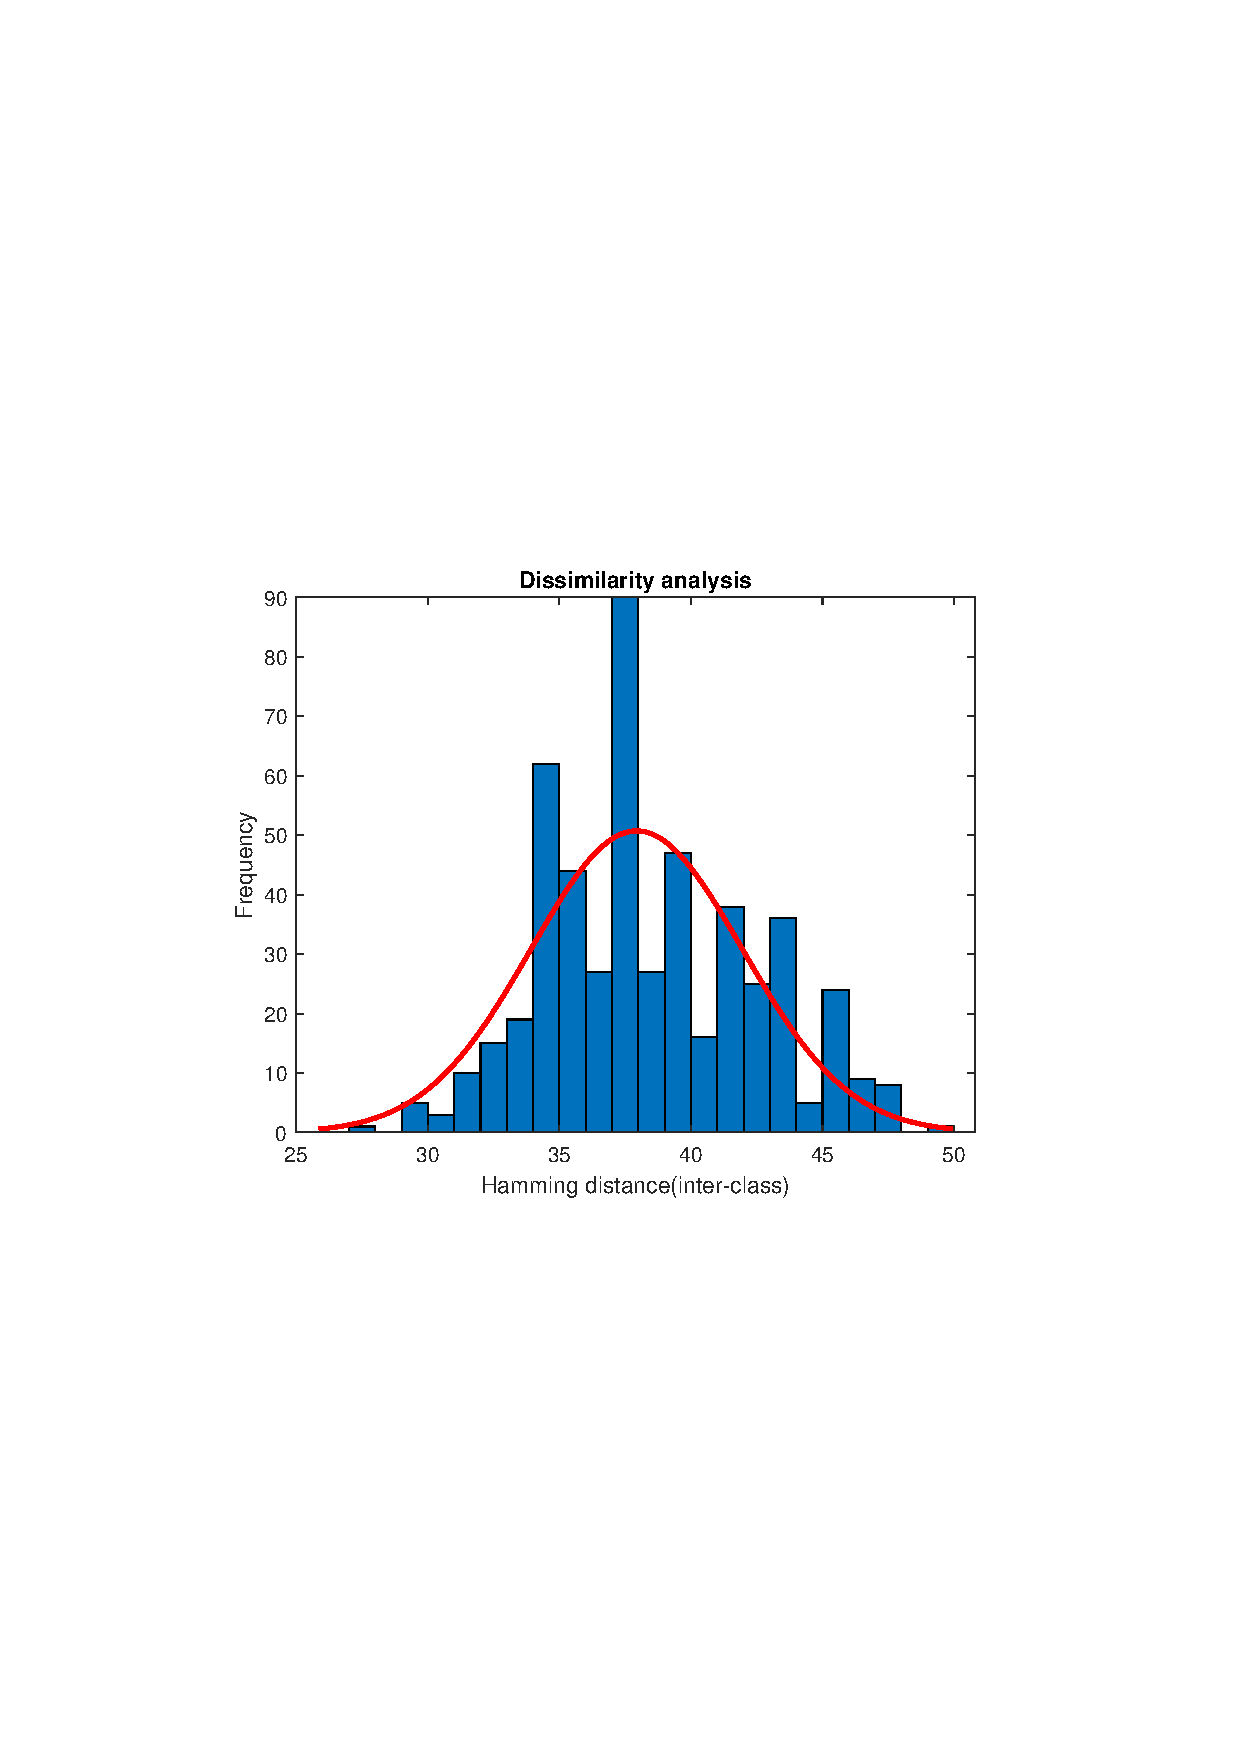
\includegraphics[width=2.5in]{disdelu1.pdf}
		\label{fig:dis1}}
	%	\subfigure[Dissimilarity analysis for texture based feature
	%	    vector.]{\centering \includegraphics[width=1.5in]{distext1.pdf}
	%	    \label{fig:dis2}}\\
	\subfigure[Dissimilarity analysis for combination of minutia and three
		texture based feature vector.]{\centering
		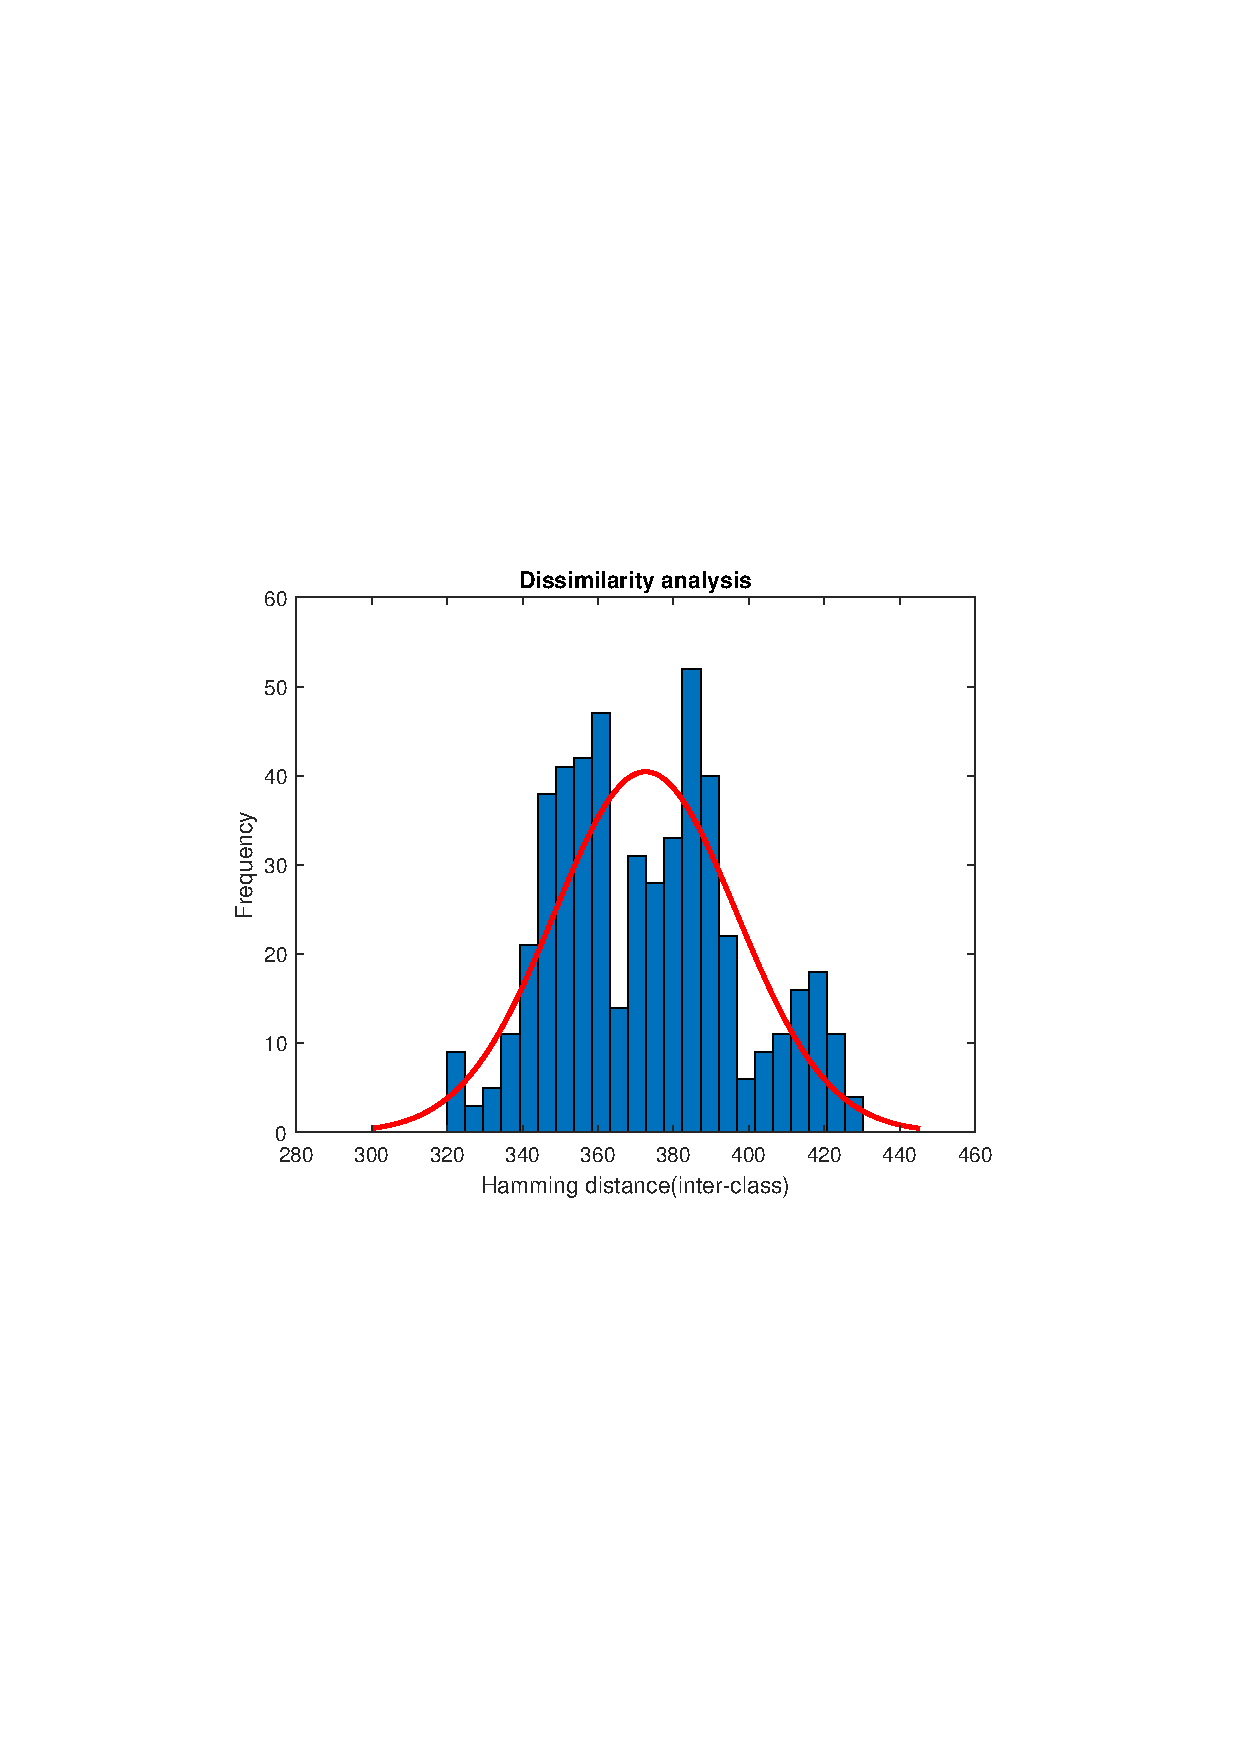
\includegraphics[width=2.5in]{dismd.pdf}
		\label{fig:dis3}} \subfigure[Dissimilarity analysis for combination of
		minutia and all four texture based feature vector.]{\centering
		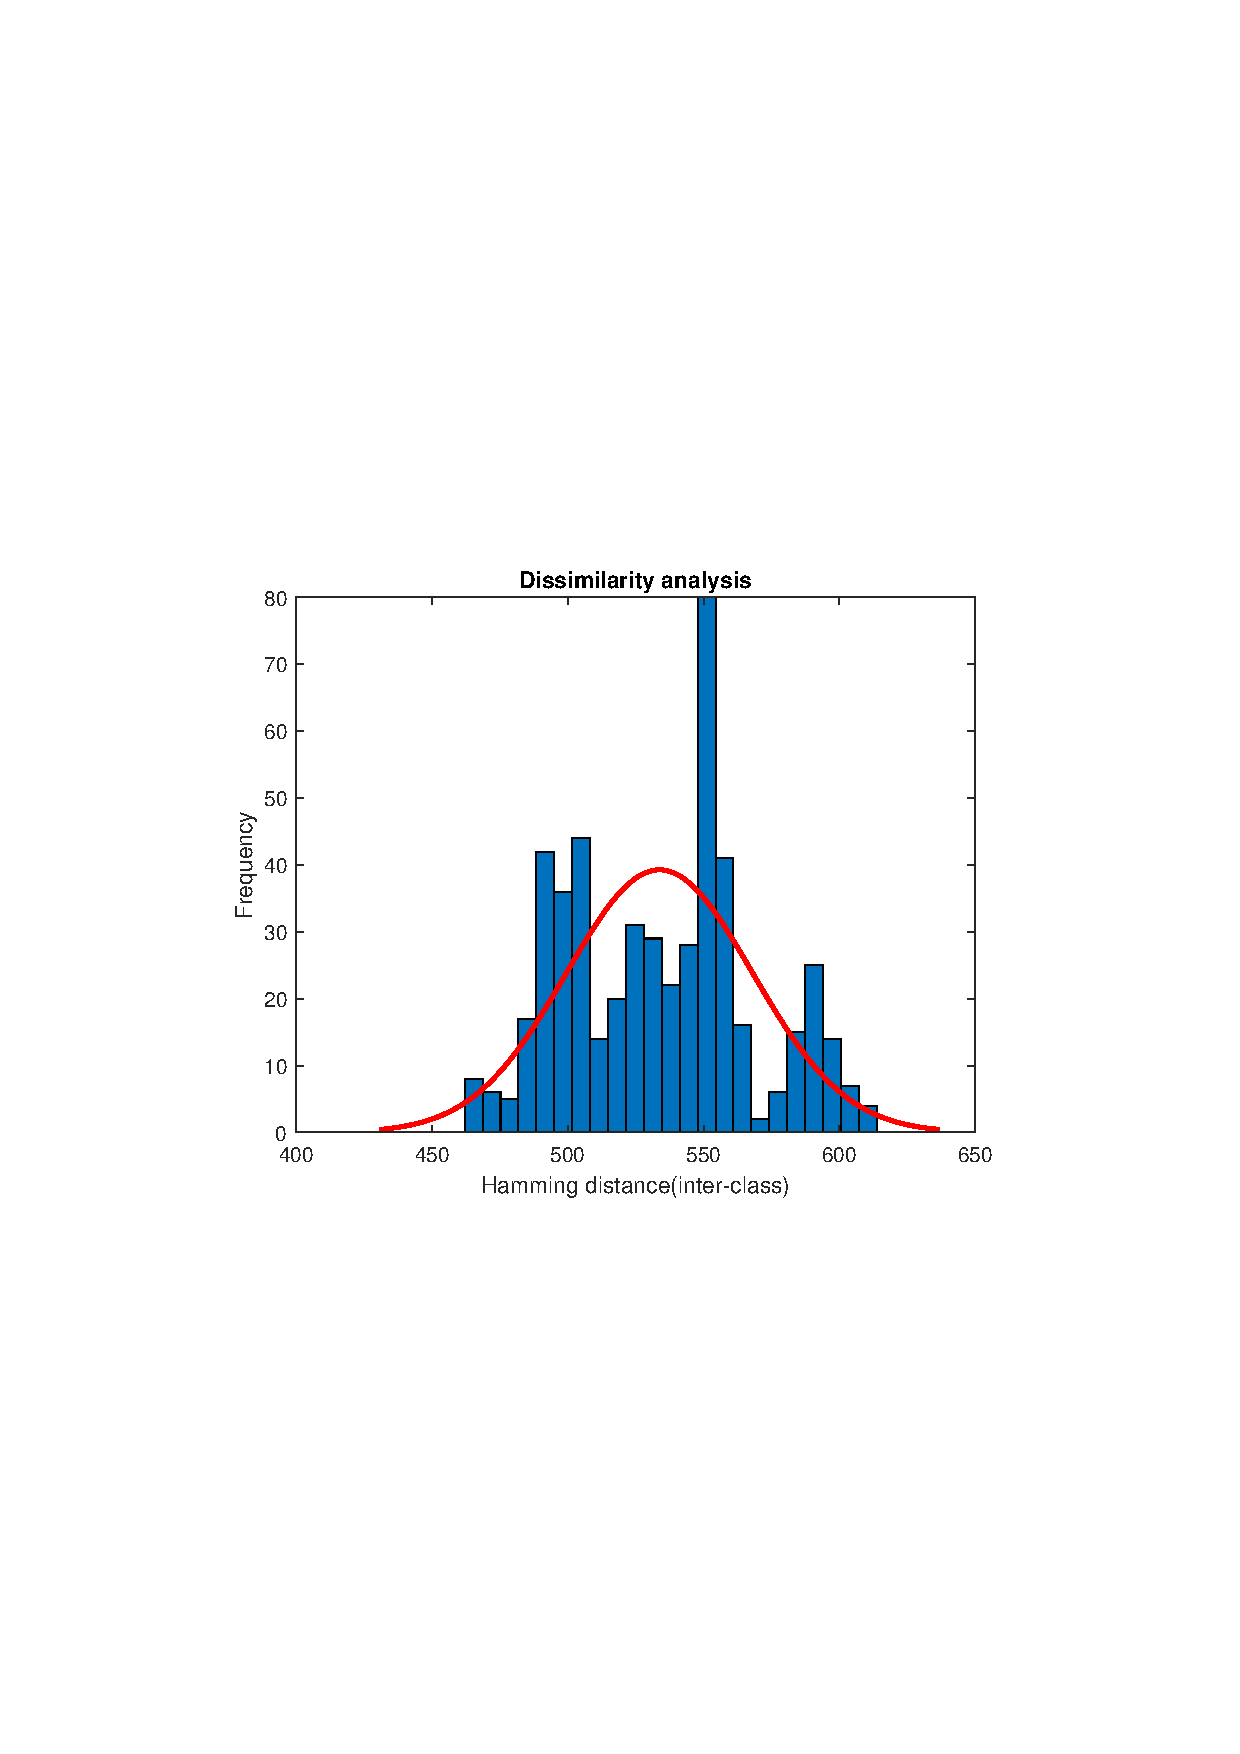
\includegraphics[width=2.5in]{distext2.pdf}
		\label{fig:dis4}}
	%	\subfloat[Consistent region.]{\centering
	%	    \includegraphics[width=1.5in]{glcm3.pdf} \label{fig:consistent3}}
	\caption{Dissimilarity analysis.}
	\label{fig:dissimilarity}
	\vspace{-4mm}
\end{figure}\par

\subsubsection{Distinctiveness analysis of keys}
In this experiment, the performance of the proposed method was analyzed through
key regeneration rate for different feature combinations, such as proposed
minutia features only (M), combination of minutia and texture features
MT1(minutia and texture1 (HCBD, GCBD, LTP)) and MT2(minutia, texture2 (HCBD,
GCBD, LTP, MTP)). The key regeneration rate (kgr) is the number of times the
key is generated for successful authentication. The key regeneration rate for
different feature combinations on different datasets is shown in Table
\ref{table:perform1}. 

\par 

\begin{table}[ht]
	\caption{Key regeneration rate using different feature(s).}
	\label{table:perform1}
	\begin{center}
		%	\resizebox{\columnwidth}{!}{
		\begin{tabular}{|l |c |c |c |}
			\hline
			Dataset                             & M-kgr   & MT1-kgr & MT2-kgr
			\\ [0.5ex]
			\hline
			FVC 2002                            & 92.43\%  & 94.44\%  & 97.22 \%
			\\
			FVC 2004                            & 92.66\%  & 93.02\%  & 96.13 \%
			\\
			High Resolution-Fingerprint(HRF) DB1 & 96.25 \% & 96.35 \% & 98.00\%
			\\
			High Resolution-Fingerprint(HRF) DB2 & 90.68 \% & 91.45 \% & 95.68 \%
			\\
			\hline
		\end{tabular}%}
	\end{center}

\end{table}

\begin{table}[!ht]
	\caption{Key regeneration rate with or without metric learning.}
	\label{table:comp}
	\begin{center}
		\resizebox{\columnwidth}{!}{
			\begin{tabular}{|l| c| c|}
				\hline
				Dataset                             & Without metric
				learning(kgr)                      & With metric learning(kgr)
				\\ [0.5ex]

				\hline
				FVC 2002                            & 91.43\%                    & 97.22\%
				\\
				FVC 2004                            & 90.66\%                    & 96.13\%
				\\
				High Resolution-Fingerprint(HRF) DB1 & 92.25 \%                   & 98.00 \%
				\\
				High Resolution-Fingerprint(HRF) DB2 & 90.88 \%                   & 95.68 \%
				\\
				\hline
			\end{tabular}}
	\end{center}

\end{table}

%\begin{table}[b] \caption{Key regeneration rate using different feature(s).}
%   \label{table:perform1} \begin{center} %   \resizebox{\columnwidth}{!}{
%   \begin{tabular}{|l c c c |} \hline Dataset & M-bkgr  & MT1-bkgr & MT1-bkgr
%   \\ [0.5ex] \hline FVC 2002  & 92.43\%  &96.09\%  & 94.44\% \\
%               FVC 2004  & 92.66\% & 93.23\% & 93.02\% \\
%               High Resolution-Fingerprint(HRF)DB1& 96.25 \%  & 97.35 \% &
%               96.35 \% \\
%               High Resolution-Fingerprint(HRF)DB2& 90.68 \%  & 92.38 \% &91.45
%               \% \\
%               \hline  
%       \end{tabular}%} \end{center}
%
%\end{table}
The missing key scenario would be the worst, as it means that either the user has
missed the secret key or the intruder knows the secret key. A new key can be
generated by changing the segment length in the key generation mechanism
described in Section~\ref{bk} or by changing the binarization scheme. So, the
proposed method ensures the revocability of the key which is not dependent on the
missing one. 
\par 

\begin{figure}[!ht]
	\centering
	\subfigure[]{
		\centering
		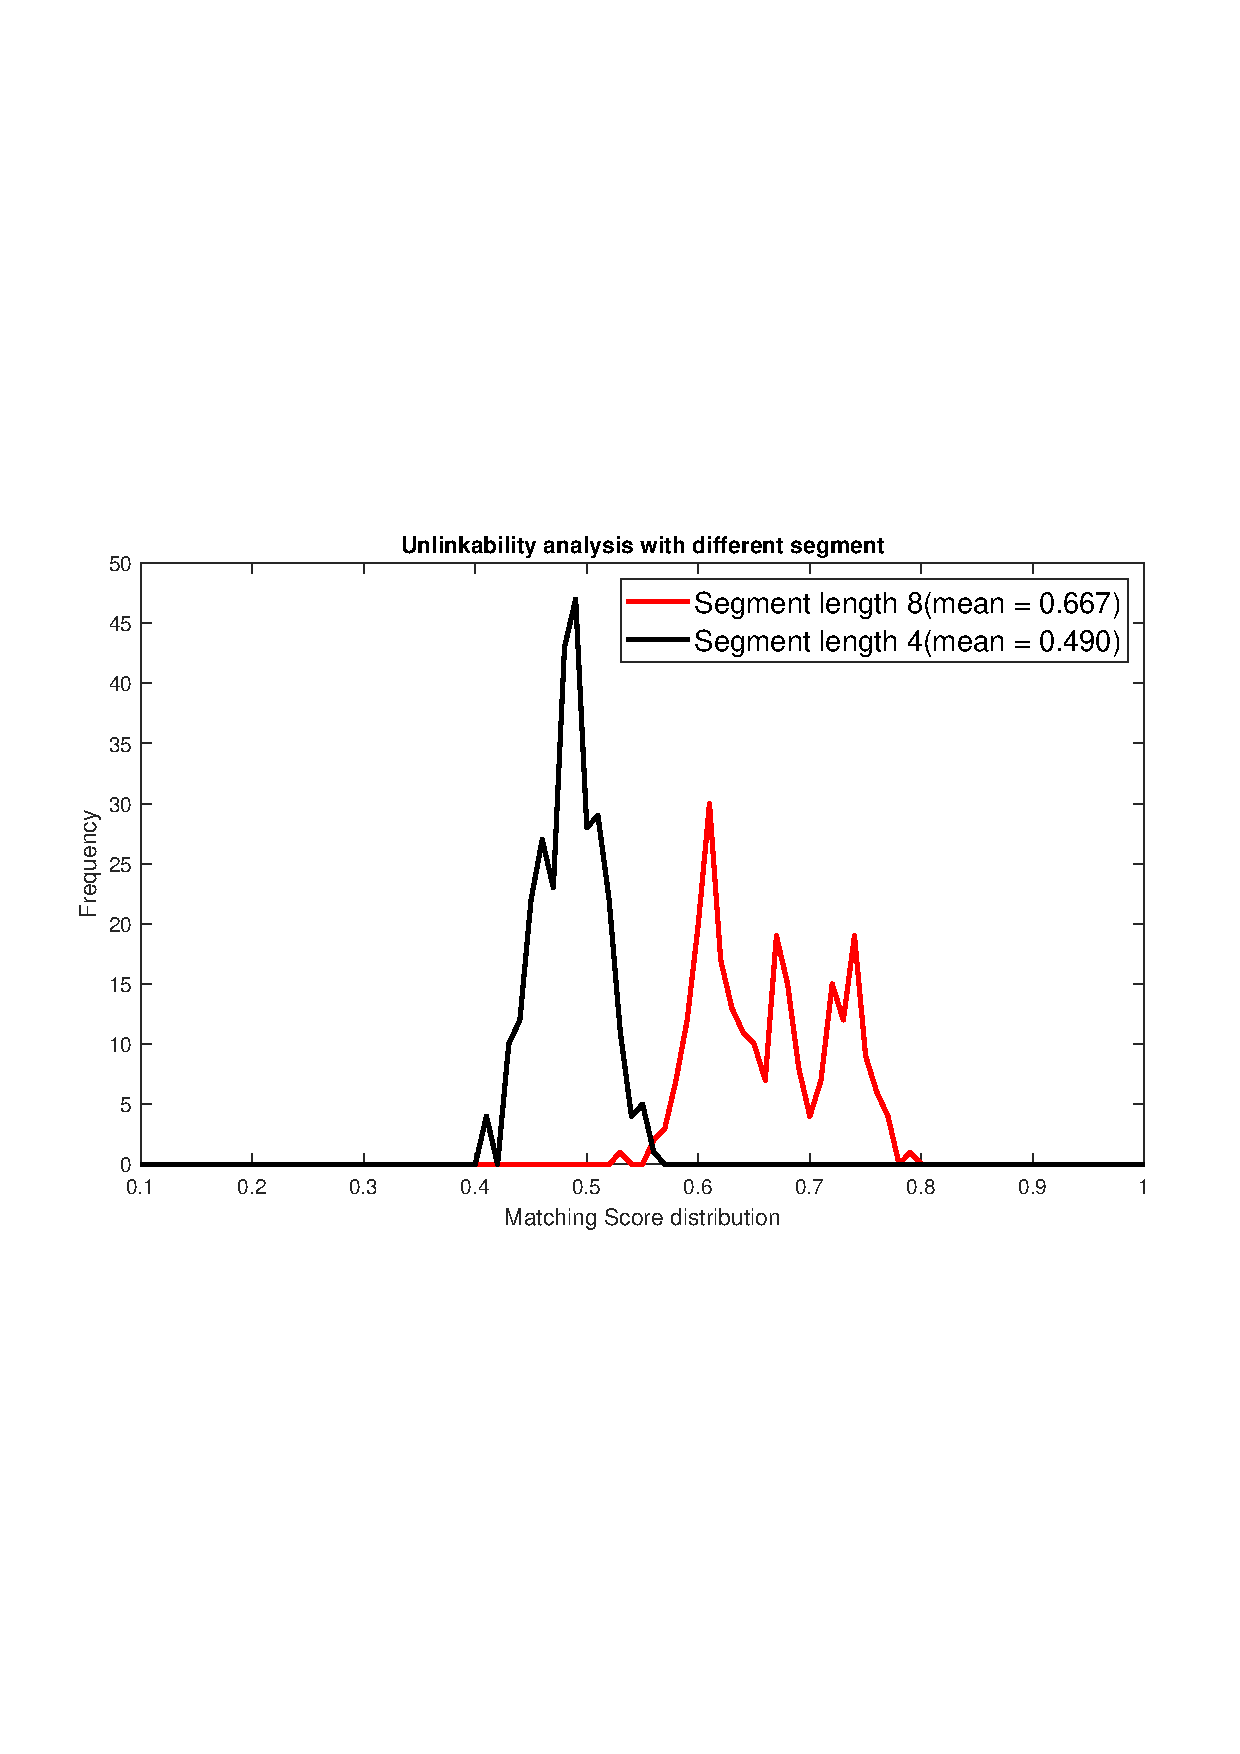
\includegraphics[width=2.5in]{segement84.pdf}
		\label{fig:quant1}} \subfigure[]{\centering
		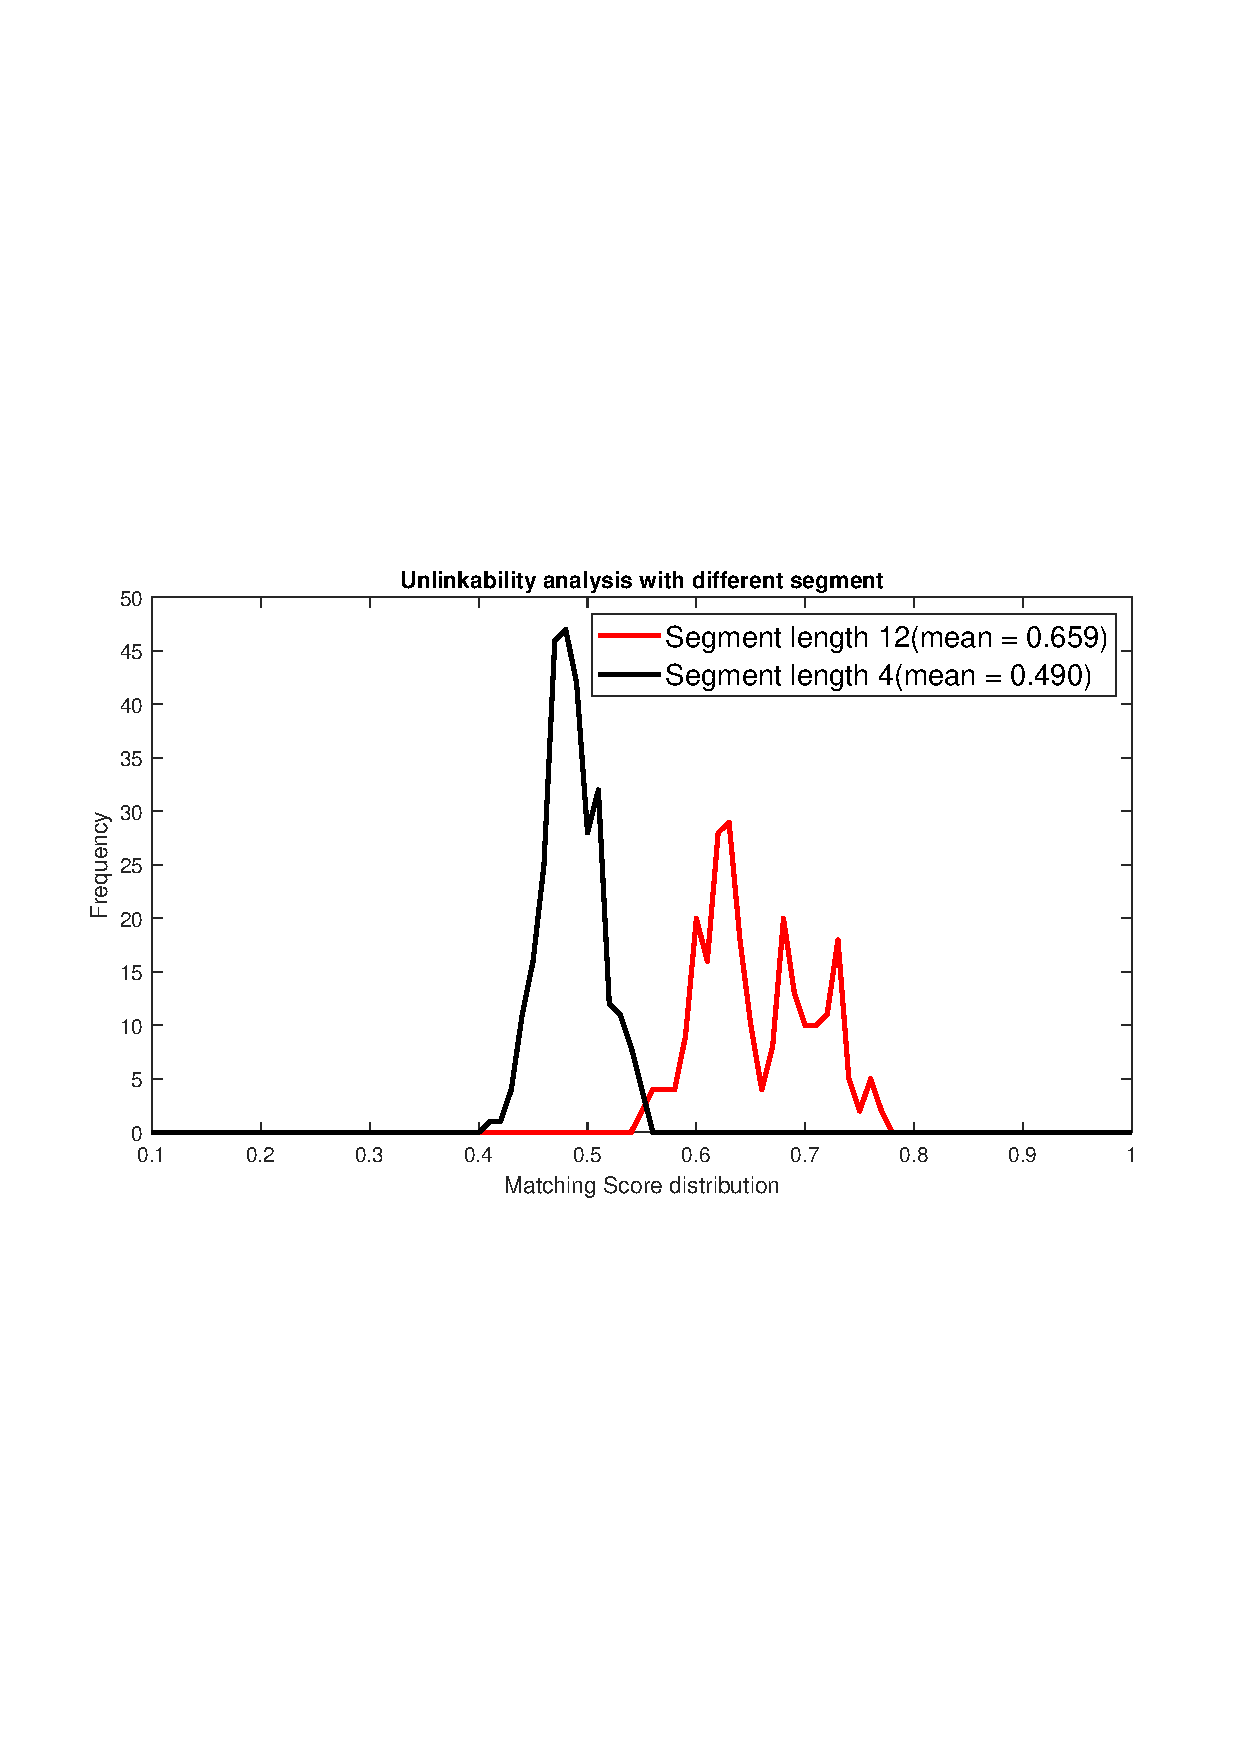
\includegraphics[width=2.7in]{segement124.pdf}
		\label{fig:quant2}}
	\caption{Illustration of  unlinkability analysis of keys generated for different segments.}
	\label{fig:quant}
	\vspace{-4mm}
\end{figure}


\subsubsection{
	Performance analysis with different fingerprint images
	}
Analysis of key regeneration rate on fingerprint images of different resolutions and
qualities were performed. For this purpose, the datasets were categorized into
four categories: 
(i) low-quality (FVC 2002 DB3, FVC 2004 DB2), 
(ii) synthetic (FVC 2002 and 2004 DB4), 
(iii) normal (other FVC 2002 and 2004 databases) and
(iv) high-resolution (HRF). The key regeneration rate of different categories of
fingerprint datasets are shown in Table \ref{table:perform2}. From the table, it is
clear that the proposed method is suitable for any kind of fingerprint image.

\begin{table}[ht]

	\caption{Key regeneration rate on various fingerprint category.}
	\label{table:perform2}
	\begin{center}
		%\resizebox{\columnwidth}{!}{
		\begin{tabular}{|l |c |c |c |}
			\hline
			Fingerprint category          & M-kgr   & MT1-kgr & MT2-kgr \\
			[0.5ex]
			\hline
			Low-quality                   & 92.69\%  & 93.24\%  & 95.52 \% \\
			Synthetic                     & 92.75\%  & 94.45\%  & 97.92\%  \\
			High Resolution               & 93.46 \% & 93.90 \% & 96.84 \% \\
			Normal resolution and quality & 93.13 \% & 93.65 \% & 96.74\%  \\
			\hline
		\end{tabular}%}
	\end{center}

\end{table}
\subsubsection{Computational complexity analysis }
The proposed method can be used to generate keys of different lengths according
to the individual cryptographic application's requirements. 
For low-cost and small
applications, key size should be less compared to large application.
~The
computational times vary in the range 152ms-600ms. 
The break-up times of
different computations are shown in Table \ref{table:timecomplexity}.
\begin{table}[!ht]
	\caption{Computational complexity analysis.}
	\label{table:timecomplexity}
	\begin{center}
		%\resizebox{\columnwidth}{!}{
		\begin{tabular}{|l |c |} \hline
			Sub-steps                                      & Computational
			time(in ms)                                                    \\
			\hline
			Pre-processing                                 & 0.534         \\
			Relative feature vector generation             & 38.212        \\
			Texture feature vector generation              & 112.245       \\
			Discriminant feature vector and key generation & 113.074       \\
			\hline
		\end{tabular}
	\end{center}
\end{table}

%The proposed minutia features can be used for all such applications. For small
% sized applications, where the key size ranges from ($64-72$), the cost of
%computation is around $52ms$. For moderate sized-applications, the key can be
%generated using texture features of size ($256-427$), and the cost of computation is
% around $152ms$. For high-end applications, a combination of feature vectors can
% be used to generate a key of length in the range ($ 720-1524$), and the cost of

%computation is around $400-600ms$.
